\documentclass[11pt]{article}
\usepackage[margin=18mm,headheight=22pt]{geometry}
\usepackage{amsmath}
\usepackage{fontspec}
\usepackage{unicode-math}
\setmainfont{NewCM10}[Extension=.otf,UprightFont=*-Book,BoldFont=*-Bold,ItalicFont=*-BookItalic,BoldItalicFont=*-BoldItalic]
\setsansfont{NewCMSans10}[Extension=.otf,UprightFont=*-Book,BoldFont=*-Bold,ItalicFont=*-BookOblique,BoldItalicFont=*-BoldOblique]
\setmathfont{NewCMMath-Book.otf}
\usepackage{xcolor}
\definecolor{FAUblue}{HTML}{04316A}
\definecolor{Paperblue}{HTML}{EEF2F7}
\definecolor{EEIgold}{HTML}{CC9C42}
\usepackage{etoolbox,enumitem,booktabs,tabularx,array,needspace,microtype}
\usepackage[most]{tcolorbox}
\usepackage{titlesec,fancyhdr}
\usepackage[hidelinks]{hyperref}
\usepackage{draftwatermark}
\SetWatermarkText{Made by Thanate Amornjiraporn (Focus)}
\SetWatermarkColor{black!7}\SetWatermarkFontSize{30pt}\SetWatermarkAngle{45}
\setlength{\parindent}{0pt}
\setlength{\parskip}{5pt}
\setlist{itemsep=2pt,topsep=3pt,leftmargin=1.6em,beginpenalty=10000,endpenalty=10000}
\raggedbottom
\clubpenalty=10000 \widowpenalty=10000 \displaywidowpenalty=10000 \interlinepenalty=10000
\setcounter{secnumdepth}{0}
\setcounter{tocdepth}{1}
\pagestyle{fancy}\fancyhf{}
\fancyhead[L]{\small\sffamily\color{FAUblue} From Fundamentals to AI Apocalypse · MEI · Exercise Sheet 5}
\fancyhead[R]{\small\sffamily Exercise 5: Worked solutions}
\fancyfoot[C]{\small\thepage}
\titleformat{\section}{\Large\bfseries\sffamily\color{FAUblue}}{}{0pt}{}
\titleformat{\subsection}{\large\bfseries\sffamily\color{FAUblue}}{}{0pt}{}
\titlespacing*{\section}{0pt}{16pt}{6pt}
\preto\section{\Needspace{8\baselineskip}}
\preto\subsection{\Needspace{6\baselineskip}}
\newtcolorbox{equationcard}[1]{colback=Paperblue,colframe=Paperblue,boxrule=0pt,arc=0pt,left=10pt,right=10pt,top=6pt,bottom=6pt,title={#1},fonttitle=\small\bfseries\sffamily,coltitle=FAUblue,before skip=8pt,after skip=8pt}
\newtcolorbox{workedbox}[1]{colback=white,colframe=EEIgold,boxrule=0pt,leftrule=3pt,arc=0pt,left=10pt,top=4pt,bottom=4pt,title={#1},fonttitle=\small\bfseries\sffamily,coltitle=FAUblue,attach title to upper={\par},before skip=8pt,after skip=8pt}
\newtcolorbox{recallbox}[1]{colback=white,colframe=FAUblue,boxrule=0pt,leftrule=3pt,arc=0pt,left=10pt,top=4pt,bottom=4pt,title={#1},fonttitle=\small\bfseries\sffamily,coltitle=FAUblue,attach title to upper={\par},before skip=8pt,after skip=8pt}
\usepackage{environ}
\newsavebox\measurebox
% Typeset the section once invisibly to measure it; start a new page if it will not fit in what is left.
\makeatletter
\newif\ifkeep@measuring
\NewEnviron{keepsection}{%
  \ifkeep@measuring \BODY \else
    \edef\keep@sec{\the\value{section}}\edef\keep@sub{\the\value{subsection}}%
    \setbox\measurebox\vbox{\hsize\linewidth\keep@measuringtrue\def\Needspace##1{}\BODY}%
    \setcounter{section}{\keep@sec}\setcounter{subsection}{\keep@sub}%
    \dimen2=\ht\measurebox \advance\dimen2\dp\measurebox
    \dimen@=\textheight
    \ifdim\pagegoal<\maxdimen
      \dimen@=\pagegoal \advance\dimen@-\pagetotal
      \ifdim\dimen2>\dimen@ \clearpage \dimen@=\textheight \fi
    \fi
    % if it fits, nothing inside may force an early break
    \ifdim\dimen2>\dimen@ \BODY \else \begingroup\def\Needspace##1{}\BODY\endgroup \fi
  \fi}
\makeatother
\newtcolorbox{notebox}{colback=Paperblue,colframe=Paperblue,boxrule=0pt,arc=0pt,left=8pt,right=8pt,top=4pt,bottom=4pt,before skip=6pt,after skip=6pt}
\newtcolorbox{plainbox}{colback=white,colframe=FAUblue,boxrule=0pt,leftrule=3pt,arc=0pt,left=10pt,right=8pt,top=4pt,bottom=4pt,before skip=6pt,after skip=8pt}
\usetikzlibrary{arrows.meta}
\title{\sffamily\bfseries\color{FAUblue}Exercise 5: Worked solutions}
\author{Mathematics for Engineers I \ensuremath{\cdot} Module 27651 \ensuremath{\cdot} Exercise Sheet 5\\[2pt]\small From Fundamentals to AI Apocalypse · personal study guide}
\date{}
\begin{document}
\maketitle
\begingroup\footnotesize\setlength{\parskip}{0pt}\tableofcontents\endgroup
\clearpage

\begin{keepsection}
\Needspace{8\baselineskip}
\section{Exercise 5.1: Polar coordinates}

\Needspace{5\baselineskip}
Convert with \textit{r} = \ensuremath{\sqrt{{x}^{2}\, +\, {y}^{2}}} and pick φ from the quadrant; for regions, ask which radii and which angles occur.

\textbf{Connected topic:} Polar coordinates (§3.6).

\begin{keepsection}
\Needspace{6\baselineskip}
\subsection{1a: Polar coordinates of (\ensuremath{-}5, 4) and (2, \ensuremath{\sqrt{7}})}

\Needspace{3\baselineskip}
Try first: compute \textit{r} by Pythagoras, then decide each point'\textit{s} quadrant before you use arctan.

\nopagebreak[4]{\small\itshape Answers: see “Exercise 5.1: Polar coordinates” under Answers at the end.}
\end{keepsection}

\begin{keepsection}
\Needspace{6\baselineskip}
\subsection{1b: Sketch the left half of the unit circle and write it in polar form}

\Needspace{3\baselineskip}
Try first: which radius do all points of \textit{x}\textsuperscript{2} + \textit{y}\textsuperscript{2} = 1 share, and which angles give \textit{x} \ensuremath{<} 0?

\nopagebreak[4]{\small\itshape Answers: see “Exercise 5.1: Polar coordinates” under Answers at the end.}
\end{keepsection}

\begin{keepsection}
\Needspace{7\baselineskip}
\subsection{1c: Sketch the ray region \textit{M} and the line \ensuremath{\ell}, and write \ensuremath{\ell} in polar form}

\Needspace{4\baselineskip}
Try first: the angles in \textit{M} span exactly π, so \textit{M} is bounded by one line through the origin. Then substitute \textit{x} = \textit{r} cos φ, \textit{y} = \textit{r} sin φ into \textit{y} = \ensuremath{-}\ensuremath{\tfrac12}\textit{x} + 2 and solve for \textit{r}.

\nopagebreak[4]{\small\itshape Answers: see “Exercise 5.1: Polar coordinates” under Answers at the end.}
\end{keepsection}
\end{keepsection}

\begin{keepsection}
\Needspace{8\baselineskip}
\section{Exercise 5.2: Arithmetic rules}

\Needspace{5\baselineskip}
Turn powers into exponentials with \textit{x}\textsuperscript{α} = e\textsuperscript{α ln \textit{x}}, and combine logarithms with ln \textit{a} + ln \textit{b} = ln(\textit{ab}).

\textbf{Connected topic:} Elementary functions (§3.5).

\begin{keepsection}
\Needspace{6\baselineskip}
\subsection{2a-i: Evaluate \ensuremath{\sqrt{\mathrm{e}^{3\, \ln \, 4}}}}

\Needspace{3\baselineskip}
Try first: write the square root as the power \ensuremath{\tfrac12} and use e\textsuperscript{ln 4} = 4.

\nopagebreak[4]{\small\itshape Answers: see “Exercise 5.2: Arithmetic rules” under Answers at the end.}
\end{keepsection}

\begin{keepsection}
\Needspace{6\baselineskip}
\subsection{2a-ii: Simplify the \textit{x}-th root expression for \textit{x} \ensuremath{>} 0}

\Needspace{3\baselineskip}
Try first: write the \textit{x}-th root as the power {\small\ensuremath{\dfrac{1}{{x}}}}, expand (2 + \textit{x})\textsuperscript{2} \ensuremath{-} 4, then divide by e\textsuperscript{\textit{x}}.

\nopagebreak[4]{\small\itshape Answers: see “Exercise 5.2: Arithmetic rules” under Answers at the end.}
\end{keepsection}

\begin{keepsection}
\Needspace{6\baselineskip}
\subsection{2b-i: Simplify ln(2x) + ln(2y) \ensuremath{-} ln \textit{z} \ensuremath{-} ln 4}

\Needspace{3\baselineskip}
Try first: collect sums of logarithms into one product and differences into one quotient.

\nopagebreak[4]{\small\itshape Answers: see “Exercise 5.2: Arithmetic rules” under Answers at the end.}
\end{keepsection}

\begin{keepsection}
\Needspace{6\baselineskip}
\subsection{2b-ii: Simplify ln(\textit{x}\textsuperscript{2} \ensuremath{-} \textit{y}\textsuperscript{2}) \ensuremath{-} ln(2(\textit{x} \ensuremath{-} \textit{y})) for \textit{x} \ensuremath{>} \textit{y}}

\Needspace{3\baselineskip}
Try first: factor \textit{x}\textsuperscript{2} \ensuremath{-} \textit{y}\textsuperscript{2} and say why both logarithms are defined.

\nopagebreak[4]{\small\itshape Answers: see “Exercise 5.2: Arithmetic rules” under Answers at the end.}
\end{keepsection}
\end{keepsection}

\begin{keepsection}
\Needspace{7\baselineskip}
\section{Exercise 5.3: Complex numbers}

\Needspace{4\baselineskip}
For quotients multiply by the conjugate of the denominator; for powers switch to polar form.

\textbf{Connected topics:} Complex arithmetic and polar form (§4.1) and Roots and powers (§4.2).

\begin{keepsection}
\Needspace{6\baselineskip}
\subsection{3a: Real part, imaginary part and magnitude of {\small\ensuremath{\dfrac{1\, +\, \mathrm{i}}{1\, -\, \mathrm{i}}}}}

\Needspace{3\baselineskip}
Try first: multiply top and bottom by 1 + i.

\nopagebreak[4]{\small\itshape Answers: see “Exercise 5.3: Complex numbers” under Answers at the end.}
\end{keepsection}

\begin{keepsection}
\Needspace{6\baselineskip}
\subsection{3b: Real part, imaginary part and magnitude of (\ensuremath{-}\ensuremath{\sqrt{5}} + i\ensuremath{\sqrt{5}})\textsuperscript{3}(1 + i)\textsuperscript{2}}

\Needspace{3\baselineskip}
Try first: write both factors in exponential form; then lengths multiply and angles add.

\nopagebreak[4]{\small\itshape Answers: see “Exercise 5.3: Complex numbers” under Answers at the end.}
\end{keepsection}

\begin{keepsection}
\Needspace{7\baselineskip}
\subsection{3c: Real part, imaginary part and magnitude of {\small\ensuremath{\dfrac{26}{12\, -\, 5\mathrm{i}}}} + {\small\ensuremath{\dfrac{39}{5\, +\, 12\mathrm{i}}}}}

\Needspace{4\baselineskip}
Try first: both denominators have magnitude squared 169 = 13\textsuperscript{2}; use that to bring the sum over one denominator.

\nopagebreak[4]{\small\itshape Answers: see “Exercise 5.3: Complex numbers” under Answers at the end.}
\end{keepsection}
\end{keepsection}

\begin{keepsection}
\Needspace{8\baselineskip}
\section{Exercise 5.4: Complex polar coordinates}

\Needspace{5\baselineskip}
Read |\textit{z} \ensuremath{-} a| as a distance, split \textit{z} = \textit{x} + iy when real and imaginary parts are compared, and keep \textit{z} \ensuremath{\neq} 0 when dividing by \textit{z}.

\textbf{Connected topic:} Complex arithmetic and polar form (§4.1).

\begin{keepsection}
\Needspace{6\baselineskip}
\subsection{4i: Sketch \{\textit{z} \ensuremath{\in} \ensuremath{\mathbb{C}} : |\textit{z} \ensuremath{-} i| = 3\}}

\Needspace{3\baselineskip}
Try first: what does |\textit{z} \ensuremath{-} a| measure in the Gaussian plane?

\nopagebreak[4]{\small\itshape Answers: see “Exercise 5.4: Complex polar coordinates” under Answers at the end.}
\end{keepsection}

\begin{keepsection}
\Needspace{6\baselineskip}
\subsection{4ii: Sketch \{\textit{z} \ensuremath{\in} \ensuremath{\mathbb{C}} : |\textit{z}| \ensuremath{-} \textit{z̅} = 1 + 2i\}}

\Needspace{3\baselineskip}
Try first: write \textit{z} = \textit{x} + iy, so \textit{z̅} = \textit{x} \ensuremath{-} iy, and compare real and imaginary parts.

\nopagebreak[4]{\small\itshape Answers: see “Exercise 5.4: Complex polar coordinates” under Answers at the end.}
\end{keepsection}

\begin{keepsection}
\Needspace{6\baselineskip}
\subsection{4iii: Sketch \{\textit{z} \ensuremath{\in} \ensuremath{\mathbb{C}} : Re({\small\ensuremath{\dfrac{1}{{z}}}}) \ensuremath{\leq} 2\}}

\Needspace{3\baselineskip}
Try first: write {\small\ensuremath{\dfrac{1}{{z}}}} = {\small\ensuremath{\dfrac{{\overline{z}}}{|{z}|^{2}}}} and multiply the inequality by |\textit{z}|\textsuperscript{2} \ensuremath{>} 0.

\nopagebreak[4]{\small\itshape Answers: see “Exercise 5.4: Complex polar coordinates” under Answers at the end.}
\end{keepsection}
\end{keepsection}

\begin{keepsection}
\Needspace{8\baselineskip}
\section{Self-Study 5.5: Polynomial division and factorisation}

\Needspace{5\baselineskip}
Guess a root among the divisors of the constant term, divide by (\textit{x} \ensuremath{-} root), and factor what is left.

\textbf{Connected topics:} Elementary functions (§3.5) and Complex polynomials (§4.3).

\begin{keepsection}
\Needspace{6\baselineskip}
\subsection{5a: Factorise \textit{x}\textsuperscript{3} \ensuremath{-} 2x\textsuperscript{2} \ensuremath{-} \textit{x} + 2}

\Needspace{3\baselineskip}
Try first: test \textit{x} = 1 and \textit{x} = \ensuremath{-}1.

\nopagebreak[4]{\small\itshape Answers: see “Self-Study 5.5: Polynomial division and factorisation” under Answers at the end.}
\end{keepsection}

\begin{keepsection}
\Needspace{6\baselineskip}
\subsection{5b: Factorise \textit{x}\textsuperscript{3} + \textit{x}\textsuperscript{2} \ensuremath{-} 2}

\Needspace{3\baselineskip}
Try first: \textit{x} = 1 is a root; after dividing, check the discriminant of the quadratic.

\nopagebreak[4]{\small\itshape Answers: see “Self-Study 5.5: Polynomial division and factorisation” under Answers at the end.}
\end{keepsection}

\begin{keepsection}
\Needspace{6\baselineskip}
\subsection{5c: Factorise \textit{x}\textsuperscript{4} \ensuremath{-} 5x\textsuperscript{2} + 4}

\Needspace{3\baselineskip}
Try first: \textit{x} = 1 and \textit{x} = \ensuremath{-}1 are both roots; divide twice (or set \textit{u} = \textit{x}\textsuperscript{2}).

\nopagebreak[4]{\small\itshape Answers: see “Self-Study 5.5: Polynomial division and factorisation” under Answers at the end.}
\end{keepsection}

\begin{keepsection}
\Needspace{7\baselineskip}
\subsection{5d: Divide 2x\textsuperscript{3} + 3x\textsuperscript{2} \ensuremath{-} 5x + 1 by \textit{x}\textsuperscript{2} + \textit{x} \ensuremath{-} 1 with remainder}

\Needspace{4\baselineskip}
Try first: the first quotient term is {\small\ensuremath{\dfrac{2\mathrm{x}^{3}}{{x}^{2}}}} = 2x; subtract and repeat until the degree drops below 2.

\nopagebreak[4]{\small\itshape Answers: see “Self-Study 5.5: Polynomial division and factorisation” under Answers at the end.}
\end{keepsection}
\end{keepsection}

\begin{keepsection}
\Needspace{8\baselineskip}
\section{Self-Study 5.6: Roots of polynomials}

\Needspace{5\baselineskip}
Build the proof of Theorem 3.7 in four steps: degrees add, \textit{x}\textsuperscript{\textit{k}} \ensuremath{-} \textit{x}\textsubscript{0}\textsuperscript{\textit{k}} has the factor \textit{x} \ensuremath{-} \textit{x}\textsubscript{0}, so a root splits off a linear factor, and induction counts the roots.

\textbf{Connected topics:} Elementary functions (§3.5) and Mathematical induction (§2.5).

\begin{keepsection}
\Needspace{7\baselineskip}
\subsection{6a: Show deg(\textit{P} \ensuremath{\cdot} \textit{Q}) = deg \textit{P} + deg \textit{Q}}

\Needspace{4\baselineskip}
Try first: which term of the product can have the highest power, and why is its coefficient not zero?

\nopagebreak[4]{\small\itshape Answers: see “Self-Study 5.6: Roots of polynomials” under Answers at the end.}
\end{keepsection}

\begin{keepsection}
\Needspace{6\baselineskip}
\subsection{6b: Show \textit{x}\textsuperscript{\textit{k}} \ensuremath{-} \textit{x}\textsubscript{0}\textsuperscript{\textit{k}} = (\textit{x} \ensuremath{-} \textit{x}\textsubscript{0}) \ensuremath{\textstyle\sum} \textit{x}\textsuperscript{\textit{k}\ensuremath{-}1\ensuremath{-}j}\textit{x}\textsubscript{0}\textsuperscript{j}}

\Needspace{3\baselineskip}
Try first: multiply out the right side and look for a telescoping sum.

\nopagebreak[4]{\small\itshape Answers: see “Self-Study 5.6: Roots of polynomials” under Answers at the end.}
\end{keepsection}

\begin{keepsection}
\Needspace{7\baselineskip}
\subsection{6c: Show \textit{P}(\textit{x}) = (\textit{x} \ensuremath{-} \textit{x}\textsubscript{0})\textit{Q}(\textit{x}) with deg \textit{Q} = \textit{n} \ensuremath{-} 1}

\Needspace{4\baselineskip}
Try first: subtract \textit{P}(\textit{x}\textsubscript{0}) = 0 from \textit{P}(\textit{x}); the constant terms cancel, and each remaining difference \textit{x}\textsuperscript{\textit{k}} \ensuremath{-} \textit{x}\textsubscript{0}\textsuperscript{\textit{k}} has the factor from 6b.

\nopagebreak[4]{\small\itshape Answers: see “Self-Study 5.6: Roots of polynomials” under Answers at the end.}
\end{keepsection}

\begin{keepsection}
\Needspace{7\baselineskip}
\subsection{6d: Prove Theorem 3.7 by induction on \textit{n}}

\Needspace{4\baselineskip}
Try first: base case degree 1; in the step, if \textit{P} has a root, split off \textit{x} \ensuremath{-} \textit{x}\textsubscript{0} with 6c and apply the hypothesis to \textit{Q}.

\nopagebreak[4]{\small\itshape Answers: see “Self-Study 5.6: Roots of polynomials” under Answers at the end.}
\end{keepsection}
\end{keepsection}

\begin{keepsection}
\Needspace{8\baselineskip}
\section{Self-Study 5.7: Difference formulas}

\Needspace{5\baselineskip}
Write \textit{x} and \textit{y} as a sum and a difference of the half-sum and half-difference, then apply the addition theorems.

\textbf{Connected topic:} Elementary functions (§3.5).

\begin{keepsection}
\Needspace{6\baselineskip}
\subsection{7a: Prove the difference formulas for sine and cosine}

\Needspace{3\baselineskip}
Try first: set \textit{a} = {\small\ensuremath{\dfrac{{x}\, +\, {y}}{2}}} and \textit{b} = {\small\ensuremath{\dfrac{{x}\, -\, {y}}{2}}}, so that \textit{x} = \textit{a} + b and \textit{y} = \textit{a} \ensuremath{-} b.

\nopagebreak[4]{\small\itshape Answers: see “Self-Study 5.7: Difference formulas” under Answers at the end.}
\end{keepsection}

\begin{keepsection}
\Needspace{6\baselineskip}
\subsection{7b: Show sin \textit{x} \ensuremath{-} sin(\textit{x} \ensuremath{-} {\small\ensuremath{\dfrac{π}{3}}}) = cos(\textit{x} \ensuremath{-} {\small\ensuremath{\dfrac{π}{6}}}) and cos \textit{x} \ensuremath{-} cos(\textit{x} + {\small\ensuremath{\dfrac{π}{3}}}) = sin(\textit{x} + {\small\ensuremath{\dfrac{π}{6}}})}

\Needspace{3\baselineskip}
Try first: put \textit{y} = \textit{x} \ensuremath{-} {\small\ensuremath{\dfrac{π}{3}}} (then \textit{y} = \textit{x} + {\small\ensuremath{\dfrac{π}{3}}}) into 7a and use sin {\small\ensuremath{\dfrac{π}{6}}} = \ensuremath{\tfrac12}.

\nopagebreak[4]{\small\itshape Answers: see “Self-Study 5.7: Difference formulas” under Answers at the end.}
\end{keepsection}

\begin{keepsection}
\Needspace{6\baselineskip}
\subsection{7c-i: Solve sin \textit{x} \ensuremath{-} sin(\textit{x} \ensuremath{-} {\small\ensuremath{\dfrac{π}{3}}}) = \ensuremath{\tfrac12} for \textit{x} \ensuremath{\in} [π, 2π]}

\Needspace{3\baselineskip}
Try first: by 7b the equation is cos(\textit{x} \ensuremath{-} {\small\ensuremath{\dfrac{π}{6}}}) = \ensuremath{\tfrac12}; work out the range of \textit{t} = \textit{x} \ensuremath{-} {\small\ensuremath{\dfrac{π}{6}}}.

\nopagebreak[4]{\small\itshape Answers: see “Self-Study 5.7: Difference formulas” under Answers at the end.}
\end{keepsection}

\begin{keepsection}
\Needspace{6\baselineskip}
\subsection{7c-ii: Solve cos \textit{x} \ensuremath{-} cos(\textit{x} + {\small\ensuremath{\dfrac{π}{3}}}) = \ensuremath{-}{\small\ensuremath{\dfrac{\sqrt{2}}{2}}} for \textit{x} \ensuremath{\in} [{\small\ensuremath{\dfrac{π}{2}}}, {\small\ensuremath{\dfrac{3π}{2}}}]}

\Needspace{3\baselineskip}
Try first: by 7b the equation is sin(\textit{x} + {\small\ensuremath{\dfrac{π}{6}}}) = \ensuremath{-}{\small\ensuremath{\dfrac{\sqrt{2}}{2}}}; find the range of \textit{t} = \textit{x} + {\small\ensuremath{\dfrac{π}{6}}}.

\nopagebreak[4]{\small\itshape Answers: see “Self-Study 5.7: Difference formulas” under Answers at the end.}
\end{keepsection}
\end{keepsection}

\begin{keepsection}
\Needspace{8\baselineskip}
\section{Self-Study 5.8: Polar coordinates}

\Needspace{5\baselineskip}
The same tools as 5.1: radius by Pythagoras, angle with the quadrant, and a line written as \textit{r} = \textit{f}(φ).

\textbf{Connected topic:} Polar coordinates (§3.6).

\begin{keepsection}
\Needspace{6\baselineskip}
\subsection{8a: Polar coordinates of (\ensuremath{-}\ensuremath{\sqrt{3}}, 1) and (\ensuremath{\sqrt{2}}, \ensuremath{-}5)}

\Needspace{3\baselineskip}
Try first: sketch both points to fix their quadrants before taking arctan.

\nopagebreak[4]{\small\itshape Answers: see “Self-Study 5.8: Polar coordinates” under Answers at the end.}
\end{keepsection}

\begin{keepsection}
\Needspace{7\baselineskip}
\subsection{8b: Describe the sketched ring section in Cartesian and polar coordinates}

\Needspace{4\baselineskip}
Try first: read off the inner radius (where \textit{M} crosses the negative \textit{x}-axis) and the outer radius (the corner at (2, 2)), then the two boundary angles.

\nopagebreak[4]{\small\itshape Answers: see “Self-Study 5.8: Polar coordinates” under Answers at the end.}
\end{keepsection}

\begin{keepsection}
\Needspace{7\baselineskip}
\subsection{8c: Write \textit{y} = 2x \ensuremath{-} 5 as \textit{r} = \textit{f}(φ) and find where \textit{f}(φ) \ensuremath{>} 0}

\Needspace{4\baselineskip}
Try first: substitute \textit{x} = \textit{r} cos φ, \textit{y} = \textit{r} sin φ and solve for \textit{r}; then find where the denominator is positive.

\nopagebreak[4]{\small\itshape Answers: see “Self-Study 5.8: Polar coordinates” under Answers at the end.}
\end{keepsection}
\end{keepsection}

\begin{keepsection}
\Needspace{7\baselineskip}
\section{Self-Study 5.9: Arithmetic rules}

\Needspace{4\baselineskip}
Change the base with log\textsubscript{2} \textit{a} = {\small\ensuremath{\dfrac{\ln \, \mathrm{a}}{\ln \, 2}}} and turn roots into powers.

\textbf{Connected topic:} Elementary functions (§3.5).

\begin{keepsection}
\Needspace{6\baselineskip}
\subsection{9a: Evaluate \ensuremath{\tfrac12} log\textsubscript{2}(4e\textsuperscript{2}) \ensuremath{-} {\small\ensuremath{\dfrac{1}{\ln \, 2}}}}

\Needspace{3\baselineskip}
Try first: split log\textsubscript{2}(4e\textsuperscript{2}) into log\textsubscript{2} 4 + 2 log\textsubscript{2} e, and write log\textsubscript{2} e = {\small\ensuremath{\dfrac{1}{\ln \, 2}}}.

\nopagebreak[4]{\small\itshape Answers: see “Self-Study 5.9: Arithmetic rules” under Answers at the end.}
\end{keepsection}

\begin{keepsection}
\Needspace{6\baselineskip}
\subsection{9b: Simplify ln(\textit{x}\textsuperscript{2/3}) \ensuremath{-} ln((\textit{x}\textsuperscript{\ensuremath{-}4})\textsuperscript{1/3}) for \textit{x} \ensuremath{>} 0, the second term being the cube root of \textit{x}\textsuperscript{\ensuremath{-}4}}

\Needspace{3\baselineskip}
Try first: write the cube root as the power {\small\ensuremath{\dfrac{1}{3}}}, then use ln(\textit{x}\textsuperscript{α}) = α ln \textit{x}.

\nopagebreak[4]{\small\itshape Answers: see “Self-Study 5.9: Arithmetic rules” under Answers at the end.}
\end{keepsection}
\end{keepsection}

\begin{keepsection}
\Needspace{7\baselineskip}
\section{Self-Study 5.10: Complex numbers}

\Needspace{4\baselineskip}
Normal form for quotients and sums, polar form for large powers.

\textbf{Connected topics:} Complex arithmetic and polar form (§4.1) and Roots and powers (§4.2).

\begin{keepsection}
\Needspace{6\baselineskip}
\subsection{10a: Real and imaginary part of {\small\ensuremath{\dfrac{10\, -\, 6\mathrm{i}}{4\, +\, 2\mathrm{i}}}}}

\Needspace{3\baselineskip}
Try first: multiply top and bottom by 4 \ensuremath{-} 2i.

\nopagebreak[4]{\small\itshape Answers: see “Self-Study 5.10: Complex numbers” under Answers at the end.}
\end{keepsection}

\begin{keepsection}
\Needspace{6\baselineskip}
\subsection{10b: Real and imaginary part of \ensuremath{\sqrt{2}}e\textsuperscript{iπ}}

\Needspace{3\baselineskip}
Try first: evaluate e\textsuperscript{iπ} with Euler'\textit{s} formula.

\nopagebreak[4]{\small\itshape Answers: see “Self-Study 5.10: Complex numbers” under Answers at the end.}
\end{keepsection}

\begin{keepsection}
\Needspace{6\baselineskip}
\subsection{10c: Real part, imaginary part and magnitude of (1 + i\ensuremath{\sqrt{2}})\textsuperscript{6}}

\Needspace{3\baselineskip}
Try first: square first, then cube the square; or use the binomial theorem.

\nopagebreak[4]{\small\itshape Answers: see “Self-Study 5.10: Complex numbers” under Answers at the end.}
\end{keepsection}

\begin{keepsection}
\Needspace{6\baselineskip}
\subsection{10d: Real part, imaginary part and magnitude of the nested quotient}

\Needspace{3\baselineskip}
Try first: simplify {\small\ensuremath{\dfrac{1}{1\, +\, \mathrm{i}}}} and {\small\ensuremath{\dfrac{1}{1\, -\, \mathrm{i}}}} first, then divide.

\nopagebreak[4]{\small\itshape Answers: see “Self-Study 5.10: Complex numbers” under Answers at the end.}
\end{keepsection}

\begin{keepsection}
\Needspace{6\baselineskip}
\subsection{10e: Real and imaginary part of (1 + i)\textsuperscript{4711}}

\Needspace{3\baselineskip}
Try first: (1 + i)\textsuperscript{8} = 16; write 4711 = 8 \ensuremath{\cdot} 588 + 7.

\nopagebreak[4]{\small\itshape Answers: see “Self-Study 5.10: Complex numbers” under Answers at the end.}
\end{keepsection}

\begin{keepsection}
\Needspace{6\baselineskip}
\subsection{10f: Real and imaginary part of ({\small\ensuremath{\dfrac{1\, +\, \mathrm{i}}{1\, -\, \mathrm{i}}}})\textsuperscript{99}}

\Needspace{3\baselineskip}
Try first: the quotient is i (Exercise 5.3a); reduce 99 modulo 4.

\nopagebreak[4]{\small\itshape Answers: see “Self-Study 5.10: Complex numbers” under Answers at the end.}
\end{keepsection}
\end{keepsection}

\begin{keepsection}
\Needspace{8\baselineskip}
\section{Self-Study 5.11: Roots of complex numbers}

\Needspace{5\baselineskip}
Write the right side in exponential form, take the real root of its length and spread the angles {\small\ensuremath{\dfrac{2π}{{n}}}} apart.

\textbf{Connected topic:} Roots and powers (§4.2).

\begin{keepsection}
\Needspace{6\baselineskip}
\subsection{11a: Solve \textit{z}\textsuperscript{6} = \ensuremath{-}64}

\Needspace{3\baselineskip}
Try first: \ensuremath{-}64 = 64e\textsuperscript{iπ}; how long is every root, and what are the six angles?

\nopagebreak[4]{\small\itshape Answers: see “Self-Study 5.11: Roots of complex numbers” under Answers at the end.}
\end{keepsection}

\begin{keepsection}
\Needspace{6\baselineskip}
\subsection{11b: Solve \textit{z}\textsuperscript{2} + 6z \ensuremath{-} 9\ensuremath{\sqrt{3}}i = 0}

\Needspace{3\baselineskip}
Try first: complete the square, (\textit{z} + 3)\textsuperscript{2} = 9 + 9\ensuremath{\sqrt{3}}i, then take both square roots.

\nopagebreak[4]{\small\itshape Answers: see “Self-Study 5.11: Roots of complex numbers” under Answers at the end.}
\end{keepsection}
\end{keepsection}

\begin{keepsection}
\Needspace{7\baselineskip}
\section{Self-Study 5.12: Trigonometric functions as polynomials}

\Needspace{4\baselineskip}
Read \textit{P}(\textit{t}) = 4t\textsuperscript{3} \ensuremath{-} 3t + 1 through \textit{t} = cos \textit{x}; zeros of \textit{P} then come from cos(3x) = \ensuremath{-}1.

\textbf{Connected topics:} Elementary functions (§3.5) and Complex polynomials (§4.3).

\begin{keepsection}
\Needspace{6\baselineskip}
\subsection{12a: Show \textit{P}(cos \textit{x}) = cos(3x) + 1 and guess a root}

\Needspace{3\baselineskip}
Try first: substitute \textit{t} = cos \textit{x} and use cos(3x) = 4 cos\textsuperscript{3} \textit{x} \ensuremath{-} 3 cos \textit{x}.

\nopagebreak[4]{\small\itshape Answers: see “Self-Study 5.12: Trigonometric functions as polynomials” under Answers at the end.}
\end{keepsection}

\begin{keepsection}
\Needspace{6\baselineskip}
\subsection{12b: Factorise \textit{P} into linear factors}

\Needspace{3\baselineskip}
Try first: divide 4t\textsuperscript{3} \ensuremath{-} 3t + 1 by \textit{t} \ensuremath{-} \ensuremath{\tfrac12} and factor the quadratic.

\nopagebreak[4]{\small\itshape Answers: see “Self-Study 5.12: Trigonometric functions as polynomials” under Answers at the end.}
\end{keepsection}

\begin{keepsection}
\Needspace{6\baselineskip}
\subsection{12c: Find all \textit{x} \ensuremath{\in} [0, 2π) with cos(3x) = \ensuremath{-}1 and explain the double root}

\Needspace{3\baselineskip}
Try first: solve 3x = π + 2kπ, then compute cos \textit{x} for each solution.

\nopagebreak[4]{\small\itshape Answers: see “Self-Study 5.12: Trigonometric functions as polynomials” under Answers at the end.}
\end{keepsection}
\end{keepsection}

\begin{keepsection}
\Needspace{8\baselineskip}
\section{Self-Study 5.13: Periodicity}

\Needspace{5\baselineskip}
To show \textit{T} is a period, compute \textit{f}(\textit{x} + \textit{T}). To show it is the smallest, find all \textit{x} with \textit{f}(\textit{x}) = \textit{f}(0) and use that every period lies among them.

\textbf{Connected topic:} Elementary functions (§3.5).

\begin{keepsection}
\Needspace{6\baselineskip}
\subsection{13a: If \textit{g} has period \textit{T}, then \textit{g}(kx) has period {\small\ensuremath{\dfrac{{T}}{{k}}}}}

\Needspace{3\baselineskip}
Try first: compute \textit{h}(\textit{x} + {\small\ensuremath{\dfrac{{T}}{{k}}}}).

\nopagebreak[4]{\small\itshape Answers: see “Self-Study 5.13: Periodicity” under Answers at the end.}
\end{keepsection}

\begin{keepsection}
\Needspace{6\baselineskip}
\subsection{13b-i: \textit{f}(\textit{x}) = cos(2x) + cos(3x) is even}

\Needspace{3\baselineskip}
Try first: use cos(\ensuremath{-}\textit{u}) = cos \textit{u}.

\nopagebreak[4]{\small\itshape Answers: see “Self-Study 5.13: Periodicity” under Answers at the end.}
\end{keepsection}

\begin{keepsection}
\Needspace{6\baselineskip}
\subsection{13b-ii: 2π is a period of \textit{f}}

\Needspace{3\baselineskip}
Try first: compute \textit{f}(\textit{x} + 2π) term by term.

\nopagebreak[4]{\small\itshape Answers: see “Self-Study 5.13: Periodicity” under Answers at the end.}
\end{keepsection}

\begin{keepsection}
\Needspace{6\baselineskip}
\subsection{13b-iii: 2π is the smallest period of \textit{f}}

\Needspace{3\baselineskip}
Try first: \textit{f}(0) = 2 and each cosine is at most 1; when is \textit{f}(\textit{x}) = 2?

\nopagebreak[4]{\small\itshape Answers: see “Self-Study 5.13: Periodicity” under Answers at the end.}
\end{keepsection}

\begin{keepsection}
\Needspace{6\baselineskip}
\subsection{13c: \textit{g}(\textit{x}) = sin(4x) + sin(6x) is odd with period π}

\Needspace{3\baselineskip}
Try first: use sin(\ensuremath{-}\textit{u}) = \ensuremath{-}sin \textit{u}, then compute \textit{g}(\textit{x} + π).

\nopagebreak[4]{\small\itshape Answers: see “Self-Study 5.13: Periodicity” under Answers at the end.}
\end{keepsection}

\begin{keepsection}
\Needspace{7\baselineskip}
\subsection{13d: cos(mx) + cos(nx) has smallest period {\small\ensuremath{\dfrac{2π}{\text{gcd}({m},\, {n})}}}}

\Needspace{4\baselineskip}
Try first: with \textit{m} = \textit{m}̃k and \textit{n} = ñ\textit{k}, show {\small\ensuremath{\dfrac{2π}{{k}}}} is a period; then solve \textit{f}(\textit{x}) = \textit{f}(0) = 2 as in 13b-iii.

\nopagebreak[4]{\small\itshape Answers: see “Self-Study 5.13: Periodicity” under Answers at the end.}
\end{keepsection}

\begin{keepsection}
\Needspace{6\baselineskip}
\subsection{13e: \textit{h}(\textit{x}) = sin \textit{x} + sin(3x): \textit{h}(\textit{x} + π) = \ensuremath{-}\textit{h}(\textit{x}), so 2π is a period and π is not}

\Needspace{3\baselineskip}
Try first: sin(\textit{u} + π) = \ensuremath{-}sin \textit{u} and 3π = π + 2π.

\nopagebreak[4]{\small\itshape Answers: see “Self-Study 5.13: Periodicity” under Answers at the end.}
\end{keepsection}
\end{keepsection}

\begin{keepsection}
\Needspace{8\baselineskip}
\section{Self-Study 5.14: Logarithm rules and mistakes}

\Needspace{5\baselineskip}
Derive the rules from e\textsuperscript{\textit{x}+\textit{y}} = e\textsuperscript{\textit{x}}e\textsuperscript{\textit{y}} and ln(e\textsuperscript{\textit{x}}) = \textit{x}; then test the false rule against the true one.

\textbf{Connected topic:} Elementary functions (§3.5).

\begin{keepsection}
\Needspace{6\baselineskip}
\subsection{14a-i: Show ln(xy) = ln \textit{x} + ln \textit{y}}

\Needspace{3\baselineskip}
Try first: write \textit{x} = e\textsuperscript{ln \textit{x}} and \textit{y} = e\textsuperscript{ln \textit{y}}.

\nopagebreak[4]{\small\itshape Answers: see “Self-Study 5.14: Logarithm rules and mistakes” under Answers at the end.}
\end{keepsection}

\begin{keepsection}
\Needspace{6\baselineskip}
\subsection{14a-ii: Show ln(\textit{x}\textsuperscript{α}) = α ln \textit{x}}

\Needspace{3\baselineskip}
Try first: use the definition \textit{x}\textsuperscript{α} := e\textsuperscript{α ln \textit{x}}.

\nopagebreak[4]{\small\itshape Answers: see “Self-Study 5.14: Logarithm rules and mistakes” under Answers at the end.}
\end{keepsection}

\begin{keepsection}
\Needspace{6\baselineskip}
\subsection{14b: When is ln(\textit{x} + \textit{y}) = ln \textit{x} + ln \textit{y} true?}

\Needspace{3\baselineskip}
Try first: the right side is ln(xy); when is ln(\textit{x} + \textit{y}) = ln(xy)?

\nopagebreak[4]{\small\itshape Answers: see “Self-Study 5.14: Logarithm rules and mistakes” under Answers at the end.}
\end{keepsection}
\end{keepsection}


\clearpage
\section{Answers}
\begin{keepsection}\subsection{Exercise 5.1: Polar coordinates}

\begin{workedbox}{1a \ensuremath{\cdot} Polar coordinates of (\ensuremath{-}5, 4) and (2, \ensuremath{\sqrt{7}})}
\Needspace{12\baselineskip}
\begin{enumerate}
\item Convert with the rules of §3.6: \textit{r} is the distance from the origin, and φ \ensuremath{\in} [0, 2π) is read from tan φ = {\small\ensuremath{\dfrac{{y}}{{x}}}} together with the signs of \textit{x} and \textit{y}.
\item \Needspace{5\baselineskip}
\textbf{(\ensuremath{-}5, 4):} \textit{r} = \ensuremath{\sqrt{25\, +\, 16}} = \ensuremath{\sqrt{41}} \ensuremath{\approx} 6.40. Here \textit{x} \ensuremath{<} 0 and \textit{y} \ensuremath{>} 0, so the point is in quadrant II and π must be added to the arctan value:

\begin{equation*}φ\, =\, \arctan \left(\dfrac{4}{-5}\right)\, +\, π\, =\, π\, -\, \arctan \left(\dfrac{4}{5}\right)\, \approx \, 2.47\end{equation*}
\item \Needspace{5\baselineskip}
\textbf{(2, \ensuremath{\sqrt{7}}):} \textit{r} = \ensuremath{\sqrt{4\, +\, 7}} = \ensuremath{\sqrt{11}} \ensuremath{\approx} 3.32. Both coordinates are positive (quadrant I), so the arctan value is already the angle:

\begin{equation*}φ\, =\, \arctan \left(\dfrac{\sqrt{7}}{2}\right)\, \approx \, 0.924\end{equation*}
\item \Needspace{6\baselineskip}
Results: (\ensuremath{-}5, 4) = (\ensuremath{\sqrt{41}}, π \ensuremath{-} arctan {\small\ensuremath{\dfrac{4}{5}}}) \ensuremath{\approx} (6.40, 2.47) and (2, \ensuremath{\sqrt{7}}) = (\ensuremath{\sqrt{11}}, arctan {\small\ensuremath{\dfrac{\sqrt{7}}{2}}}) \ensuremath{\approx} (3.32, 0.924).

Check: 6.40 \ensuremath{\cdot} cos 2.47 \ensuremath{\approx} \ensuremath{-}5.0 and 6.40 \ensuremath{\cdot} sin 2.47 \ensuremath{\approx} 4.0. A common slip is to stop at arctan(\ensuremath{-}0.8) \ensuremath{\approx} \ensuremath{-}0.67, which points into quadrant IV.
\end{enumerate}
\end{workedbox}

\end{keepsection}
\begin{keepsection}\subsection{Exercise 5.1: Polar coordinates}

\begin{workedbox}{1b \ensuremath{\cdot} Sketch the left half of the unit circle and write it in polar form}
\Needspace{8\baselineskip}
\begin{enumerate}
\item \textit{x}\textsuperscript{2} + \textit{y}\textsuperscript{2} = 1 is the unit circle, so every point of \textit{M} has \textit{r} = 1.
\item \Needspace{5\baselineskip}
On the unit circle \textit{x} = cos φ, and cos φ \ensuremath{<} 0 exactly for {\small\ensuremath{\dfrac{π}{2}}} \ensuremath{<} φ \ensuremath{<} {\small\ensuremath{\dfrac{3π}{2}}}. The endpoints (0, \ensuremath{\pm}1) have \textit{x} = 0 and are excluded.

\Needspace{8\baselineskip}
\begin{equation*}{M}\, =\, \{({r},\, φ)\, :\, {r}\, =\, 1,\, \dfrac{π}{2}\, <\, φ\, <\, \dfrac{3π}{2}\}\end{equation*}

\Needspace{14\baselineskip}
\begin{center}
\begin{minipage}[t]{0.950\linewidth}\centering
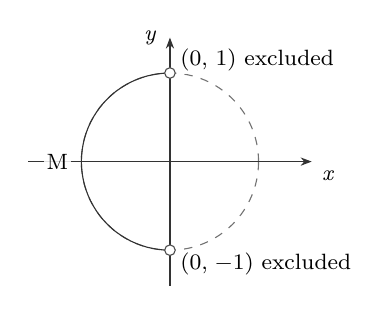
\begin{tikzpicture}[line join=round]
\draw[black!55,dashed] (2.232,-2.007) circle (1.125);
\draw[-{Stealth[length=4pt]},black!80] (0.432,-2.007) -- (4.032,-2.007);
\node[anchor=west,fill=white,fill opacity=0.85,text opacity=1,inner sep=1pt,font=\footnotesize] at (4.122,-2.187) {\textit{x}};
\draw[-{Stealth[length=4pt]},black!80] (2.232,-3.582) -- (2.232,-0.432);
\node[anchor=east,fill=white,fill opacity=0.85,text opacity=1,inner sep=1pt,font=\footnotesize] at (2.106,-0.432) {\textit{y}};
\filldraw[draw=black!80] (2.232,-0.882) -- (2.158,-0.884) -- (2.085,-0.892) -- (2.013,-0.904) -- (1.941,-0.920) -- (1.870,-0.942) -- (1.801,-0.968) -- (1.734,-0.998) -- (1.670,-1.033) -- (1.607,-1.072) -- (1.547,-1.114) -- (1.490,-1.161) -- (1.437,-1.212) -- (1.386,-1.265) -- (1.339,-1.322) -- (1.297,-1.382) -- (1.258,-1.444) -- (1.223,-1.509) -- (1.193,-1.576) -- (1.167,-1.645) -- (1.145,-1.716) -- (1.129,-1.788) -- (1.117,-1.860) -- (1.109,-1.933) -- (1.107,-2.007) -- (1.109,-2.081) -- (1.117,-2.154) -- (1.129,-2.226) -- (1.145,-2.298) -- (1.167,-2.369) -- (1.193,-2.438) -- (1.223,-2.505) -- (1.258,-2.569) -- (1.297,-2.632) -- (1.339,-2.692) -- (1.386,-2.749) -- (1.437,-2.802) -- (1.490,-2.853) -- (1.547,-2.900) -- (1.607,-2.942) -- (1.669,-2.981) -- (1.734,-3.016) -- (1.801,-3.046) -- (1.870,-3.072) -- (1.941,-3.094) -- (2.013,-3.110) -- (2.085,-3.122) -- (2.158,-3.130) -- (2.232,-3.132) -- (2.232,-3.132) -- (2.158,-3.130) -- (2.085,-3.122) -- (2.013,-3.110) -- (1.941,-3.094) -- (1.870,-3.072) -- (1.801,-3.046) -- (1.734,-3.016) -- (1.669,-2.981) -- (1.607,-2.942) -- (1.547,-2.900) -- (1.490,-2.853) -- (1.437,-2.802) -- (1.386,-2.749) -- (1.339,-2.692) -- (1.297,-2.632) -- (1.258,-2.569) -- (1.223,-2.505) -- (1.193,-2.438) -- (1.167,-2.369) -- (1.145,-2.298) -- (1.129,-2.226) -- (1.117,-2.154) -- (1.109,-2.081) -- (1.107,-2.007) -- (1.109,-1.933) -- (1.117,-1.860) -- (1.129,-1.788) -- (1.145,-1.716) -- (1.167,-1.645) -- (1.193,-1.576) -- (1.223,-1.509) -- (1.258,-1.444) -- (1.297,-1.382) -- (1.339,-1.322) -- (1.386,-1.265) -- (1.437,-1.212) -- (1.490,-1.161) -- (1.547,-1.114) -- (1.607,-1.072) -- (1.670,-1.033) -- (1.734,-0.998) -- (1.801,-0.968) -- (1.870,-0.942) -- (1.941,-0.920) -- (2.013,-0.904) -- (2.085,-0.892) -- (2.158,-0.884) -- (2.232,-0.882) -- cycle;
\draw[draw=black!70,fill=white] (2.232,-0.882) circle (0.067);
\draw[draw=black!70,fill=white] (2.232,-3.132) circle (0.067);
\node[anchor=east,fill=white,fill opacity=0.85,text opacity=1,inner sep=1pt,font=\footnotesize] at (0.981,-2.007) {M};
\node[anchor=west,fill=white,fill opacity=0.85,text opacity=1,inner sep=1pt,font=\footnotesize] at (2.322,-0.720) {(0, 1) excluded};
\node[anchor=west,fill=white,fill opacity=0.85,text opacity=1,inner sep=1pt,font=\footnotesize] at (2.322,-3.312) {(0, \ensuremath{-}1) excluded};
\end{tikzpicture}\par\smallskip{\small\raggedright \textbf{The set \textit{M}.} The solid arc is the left half of the unit circle; the dashed right half and the two open endpoints on the \textit{y}-axis do not belong to \textit{M}.\par}\end{minipage}
\end{center}
\item Check: φ = π gives (\ensuremath{-}1, 0), which has \textit{x} \ensuremath{<} 0 and lies on the circle.
\end{enumerate}
\end{workedbox}

\end{keepsection}
\begin{keepsection}\subsection{Exercise 5.1: Polar coordinates}

\begin{workedbox}{1c \ensuremath{\cdot} Sketch the ray region \textit{M} and the line \ensuremath{\ell}, and write \ensuremath{\ell} in polar form}
\Needspace{20\baselineskip}
\begin{enumerate}
\item \textbf{The set \textit{M}.} \textit{M} collects all rays from the origin with angles strictly between 0.85π and 1.85π, plus the origin itself (\textit{r} = 0). The two boundary angles point in opposite directions along one line through the origin, and tan(0.85π) \ensuremath{\approx} \ensuremath{-}\ensuremath{\tfrac12} says that line is \textit{y} = \ensuremath{-}\ensuremath{\tfrac12}\textit{x}.
\item \Needspace{5\baselineskip}
The middle angle 1.35π points down and to the left, so \textit{M} is the open half-plane below that line, together with the origin:

\begin{equation*}{M}\, =\, \{({x},\, {y})\, :\, {y}\, <\, -\tfrac{1}{2}{x}\}\, \cup \, \{(0,\, 0)\}\end{equation*}
\item \Needspace{4\baselineskip}
\textbf{The line \ensuremath{\ell} in polar form.} Substitute \textit{x} = \textit{r} cos φ and \textit{y} = \textit{r} sin φ into \textit{y} = \ensuremath{-}\ensuremath{\tfrac12}\textit{x} + 2:

\Needspace{4\baselineskip}
\begin{equation*}{r}\, \sin \, φ\, =\, -\tfrac{1}{2}\, {r}\, \cos \, φ\, +\, 2\, \Leftrightarrow \, {r}(2\, \sin \, φ\, +\, \cos \, φ)\, =\, 4\end{equation*}

\Needspace{4\baselineskip}
Wherever 2 sin φ + cos φ \ensuremath{>} 0 this gives

\begin{equation*}{r}\, =\, {f}(φ)\, =\, \dfrac{4}{2\, \sin \, φ\, +\, \cos \, φ}\end{equation*}
\item \Needspace{6\baselineskip}
\textbf{Which rays meet \ensuremath{\ell}?} A radius must be positive, so a ray at angle φ meets \ensuremath{\ell} exactly when 2 sin φ + cos φ \ensuremath{>} 0. The denominator vanishes when tan φ = \ensuremath{-}\ensuremath{\tfrac12}, that is at φ \ensuremath{\approx} 0.85π and φ \ensuremath{\approx} 1.85π (exactly π \ensuremath{-} arctan \ensuremath{\tfrac12} and its partner one half-turn later); between those angles it is negative.

\Needspace{8\baselineskip}
\begin{equation*}\ell \, =\, \{({r},\, φ)\, :\, {r}\, =\, \dfrac{4}{2\, \sin \, φ\, +\, \cos \, φ},\, φ\, \in \, [0,\, 0.85π)\, \cup \, (1.85π,\, 2π)\}\end{equation*}

\Needspace{14\baselineskip}
\begin{center}
\begin{minipage}[t]{0.950\linewidth}\centering
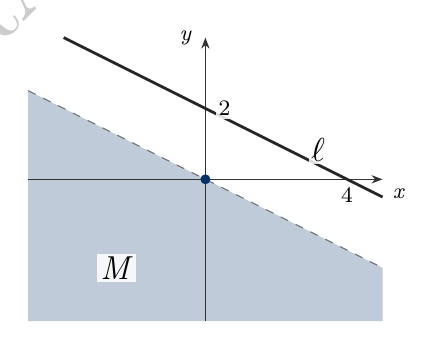
\begin{tikzpicture}[line join=round]
\fill[FAUblue!25] (0.432,-1.107) -- (4.932,-3.357) -- (4.932,-4.032) -- (0.432,-4.032) -- cycle;
\draw[-{Stealth[length=4pt]},black!80] (0.432,-2.232) -- (4.932,-2.232);
\node[anchor=west,fill=white,fill opacity=0.85,text opacity=1,inner sep=1pt,font=\footnotesize] at (5.022,-2.412) {\textit{x}};
\draw[-{Stealth[length=4pt]},black!80] (2.682,-4.032) -- (2.682,-0.432);
\node[anchor=east,fill=white,fill opacity=0.85,text opacity=1,inner sep=1pt,font=\footnotesize] at (2.556,-0.432) {\textit{y}};
\draw[black!55,dashed] (0.432,-1.107) -- (4.932,-3.357);
\draw[black!85,line width=1pt] (0.882,-0.432) -- (4.932,-2.457);
\fill[FAUblue] (2.682,-2.232) circle (0.063);
\node[fill=white,fill opacity=0.85,text opacity=1,inner sep=1pt,font=\large] at (1.557,-3.357) {\textit{M}};
\node[fill=white,fill opacity=0.85,text opacity=1,inner sep=1pt,font=\large] at (4.122,-1.854) {\textit{\ensuremath{\ell}}};
\node[anchor=west,fill=white,fill opacity=0.85,text opacity=1,inner sep=1pt,font=\footnotesize] at (2.808,-1.332) {2};
\node[fill=white,fill opacity=0.85,text opacity=1,inner sep=1pt,font=\footnotesize] at (4.482,-2.430) {4};
\end{tikzpicture}\par\smallskip{\small\raggedright \textbf{\textit{M} and \ensuremath{\ell}.} The shaded half-plane below the dashed line \textit{y} = \ensuremath{-}\ensuremath{\tfrac12}\textit{x} (not included) plus the origin is \textit{M}. The solid line \ensuremath{\ell} is parallel to that boundary, two units higher.\par}\end{minipage}
\end{center}
\item Check: φ = {\small\ensuremath{\dfrac{π}{2}}} gives \textit{r} = {\small\ensuremath{\dfrac{4}{2}}} = 2, the point (0, 2), which lies on \ensuremath{\ell}. Notice that every ray of \textit{M} has an angle where \textit{f} is not positive: no ray of \textit{M} reaches \ensuremath{\ell}, which fits the picture, since \ensuremath{\ell} runs parallel to \textit{M}'\textit{s} boundary on the other side.
\end{enumerate}
\end{workedbox}

\end{keepsection}
\begin{keepsection}\subsection{Exercise 5.2: Arithmetic rules}

\begin{workedbox}{2a-i \ensuremath{\cdot} Evaluate \ensuremath{\sqrt{\mathrm{e}^{3\, \ln \, 4}}}}
\Needspace{5\baselineskip}
\begin{enumerate}
\item \Needspace{4\baselineskip}
A square root is the power \ensuremath{\tfrac12}, and powers of e multiply exponents:

\begin{equation*}\sqrt{\mathrm{e}^{3\, \ln \, 4}}\, =\, (\mathrm{e}^{3\, \ln \, 4})^{1/2}\, =\, \mathrm{e}^{(3/2)\, \ln \, 4}\, =\, (\mathrm{e}^{\ln \, 4})^{3/2}\, =\, 4^{3/2}\end{equation*}
\item \Needspace{4\baselineskip}
4\textsuperscript{3/2} = (\ensuremath{\sqrt{4}})\textsuperscript{3} = 2\textsuperscript{3} = 8.

Check: e\textsuperscript{3 ln 4} = 4\textsuperscript{3} = 64, and \ensuremath{\sqrt{64}} = 8.
\end{enumerate}
\end{workedbox}

\end{keepsection}
\begin{keepsection}\subsection{Exercise 5.2: Arithmetic rules}

\begin{workedbox}{2a-ii \ensuremath{\cdot} Simplify the \textit{x}-th root expression for \textit{x} \ensuremath{>} 0}
\Needspace{6\baselineskip}
\begin{enumerate}
\item The \textit{x}-th root is the power {\small\ensuremath{\dfrac{1}{{x}}}}, so the numerator is e to the exponent {\small\ensuremath{\dfrac{(2\, +\, {x})^{2}\, -\, 4}{{x}}}}.
\item Expand: (2 + \textit{x})\textsuperscript{2} \ensuremath{-} 4 = \textit{x}\textsuperscript{2} + 4x, and {\small\ensuremath{\dfrac{{x}^{2}\, +\, 4\mathrm{x}}{{x}}}} = \textit{x} + 4 because \textit{x} \ensuremath{>} 0.
\item \Needspace{4\baselineskip}
Dividing by e\textsuperscript{\textit{x}} subtracts \textit{x} from the exponent:

\Needspace{4\baselineskip}
\begin{equation*}\dfrac{\mathrm{e}^{{x}\, +\, 4}}{\mathrm{e}^{{x}}}\, =\, \mathrm{e}^{4}\end{equation*}

The answer does not depend on \textit{x}. Check with \textit{x} = 1: the root is e\textsuperscript{5}, and e\textsuperscript{5} ÷ e = e\textsuperscript{4}.
\end{enumerate}
\end{workedbox}

\end{keepsection}
\begin{keepsection}\subsection{Exercise 5.2: Arithmetic rules}

\begin{workedbox}{2b-i \ensuremath{\cdot} Simplify ln(2x) + ln(2y) \ensuremath{-} ln \textit{z} \ensuremath{-} ln 4}
\Needspace{5\baselineskip}
\begin{enumerate}
\item \Needspace{4\baselineskip}
For positive arguments ln \textit{a} + ln \textit{b} = ln(ab) and ln \textit{a} \ensuremath{-} ln \textit{b} = ln {\small\ensuremath{\dfrac{\mathrm{a}}{\mathrm{b}}}}:

\begin{equation*}\ln (2\mathrm{x})\, +\, \ln (2\mathrm{y})\, -\, \ln \, {z}\, -\, \ln \, 4\, =\, \ln \, \dfrac{2\mathrm{x}\, \cdot \, 2\mathrm{y}}{4\mathrm{z}}\, =\, \ln \, \dfrac{\text{xy}}{{z}}\end{equation*}
\item Check with \textit{x} = \textit{y} = \textit{z} = 1: the left side is 2 ln 2 \ensuremath{-} 0 \ensuremath{-} ln 4 = 0 = ln 1.
\end{enumerate}
\end{workedbox}

\end{keepsection}
\begin{keepsection}\subsection{Exercise 5.2: Arithmetic rules}

\begin{workedbox}{2b-ii \ensuremath{\cdot} Simplify ln(\textit{x}\textsuperscript{2} \ensuremath{-} \textit{y}\textsuperscript{2}) \ensuremath{-} ln(2(\textit{x} \ensuremath{-} \textit{y})) for \textit{x} \ensuremath{>} \textit{y}}
\Needspace{7\baselineskip}
\begin{enumerate}
\item Since \textit{x} \ensuremath{>} \textit{y} \ensuremath{>} 0, both \textit{x} \ensuremath{-} \textit{y} and \textit{x} + \textit{y} are positive, so both arguments are positive and the rules apply.
\item \Needspace{4\baselineskip}
Factor the difference of squares and cancel \textit{x} \ensuremath{-} \textit{y} \ensuremath{\neq} 0:

\begin{equation*}\ln ({x}^{2}\, -\, {y}^{2})\, -\, \ln (2({x}\, -\, {y}))\, =\, \ln \, \dfrac{({x}\, -\, {y})({x}\, +\, {y})}{2({x}\, -\, {y})}\, =\, \ln \, \dfrac{{x}\, +\, {y}}{2}\end{equation*}
\item Check with \textit{x} = 3, \textit{y} = 1: ln 8 \ensuremath{-} ln 4 = ln 2 = ln {\small\ensuremath{\dfrac{3\, +\, 1}{2}}}.
\end{enumerate}
\end{workedbox}

\end{keepsection}
\begin{keepsection}\subsection{Exercise 5.3: Complex numbers}

\begin{workedbox}{3a \ensuremath{\cdot} Real part, imaginary part and magnitude of {\small\ensuremath{\dfrac{1\, +\, \mathrm{i}}{1\, -\, \mathrm{i}}}}}
\Needspace{6\baselineskip}
\begin{enumerate}
\item \Needspace{4\baselineskip}
The denominator'\textit{s} conjugate is 1 + i, and (1 \ensuremath{-} i)(1 + i) = 1 \ensuremath{-} i\textsuperscript{2} = 2:

\begin{equation*}\dfrac{1\, +\, \mathrm{i}}{1\, -\, \mathrm{i}}\, =\, \dfrac{(1\, +\, \mathrm{i})^{2}}{2}\, =\, \dfrac{1\, +\, 2\mathrm{i}\, +\, \mathrm{i}^{2}}{2}\, =\, \dfrac{2\mathrm{i}}{2}\, =\, \mathrm{i}\end{equation*}
\item \Needspace{4\baselineskip}
So Re = 0, Im = 1 and |i| = 1.

Check: |1 + i| = |1 \ensuremath{-} i| = \ensuremath{\sqrt{2}}, so the quotient must have magnitude 1.
\end{enumerate}
\end{workedbox}

\end{keepsection}
\begin{keepsection}\subsection{Exercise 5.3: Complex numbers}

\begin{workedbox}{3b \ensuremath{\cdot} Real part, imaginary part and magnitude of (\ensuremath{-}\ensuremath{\sqrt{5}} + i\ensuremath{\sqrt{5}})\textsuperscript{3}(1 + i)\textsuperscript{2}}
\Needspace{11\baselineskip}
\begin{enumerate}
\item \Needspace{4\baselineskip}
\ensuremath{-}\ensuremath{\sqrt{5}} + i\ensuremath{\sqrt{5}} = \ensuremath{\sqrt{5}}(\ensuremath{-}1 + i). Its length is \ensuremath{\sqrt{5}} \ensuremath{\cdot} \ensuremath{\sqrt{2}} = \ensuremath{\sqrt{10}}, and it lies in quadrant II at angle {\small\ensuremath{\dfrac{3π}{4}}}:

\begin{equation*}-\sqrt{5}\, +\, \mathrm{i}\sqrt{5}\, =\, \sqrt{10}\, \mathrm{e}^{\mathrm{i}3π/4}\end{equation*}
\item Cube it with de Moivre: the length becomes (\ensuremath{\sqrt{10}})\textsuperscript{3} = 10\ensuremath{\sqrt{10}} and the angle 3 \ensuremath{\cdot} {\small\ensuremath{\dfrac{3π}{4}}} = {\small\ensuremath{\dfrac{9π}{4}}}, which is {\small\ensuremath{\dfrac{π}{4}}} after removing a full turn.
\item \Needspace{4\baselineskip}
(1 + i)\textsuperscript{2} = 1 + 2i \ensuremath{-} 1 = 2i = 2e\textsuperscript{iπ/2}. Multiply lengths and add angles:

\begin{equation*}10\sqrt{10}\, \mathrm{e}^{\mathrm{i}π/4}\, \cdot \, 2\mathrm{e}^{\mathrm{i}π/2}\, =\, 20\sqrt{10}\, \mathrm{e}^{\mathrm{i}3π/4}\, =\, 20\sqrt{10}\left(-\dfrac{\sqrt{2}}{2}\, +\, \mathrm{i}\dfrac{\sqrt{2}}{2}\right)\, =\, -20\sqrt{5}\, +\, 20\sqrt{5}\mathrm{i}\end{equation*}
\item \Needspace{4\baselineskip}
So Re = \ensuremath{-}20\ensuremath{\sqrt{5}} \ensuremath{\approx} \ensuremath{-}44.7, Im = 20\ensuremath{\sqrt{5}} \ensuremath{\approx} 44.7, and the magnitude is 20\ensuremath{\sqrt{10}} \ensuremath{\approx} 63.2.

Check: |\ensuremath{-}20\ensuremath{\sqrt{5}} + 20\ensuremath{\sqrt{5}}i| = 20\ensuremath{\sqrt{5}} \ensuremath{\cdot} \ensuremath{\sqrt{2}} = 20\ensuremath{\sqrt{10}}, matching the product of the lengths 10\ensuremath{\sqrt{10}} \ensuremath{\cdot} 2.
\end{enumerate}
\end{workedbox}

\end{keepsection}
\begin{keepsection}\subsection{Exercise 5.3: Complex numbers}

\begin{workedbox}{3c \ensuremath{\cdot} Real part, imaginary part and magnitude of {\small\ensuremath{\dfrac{26}{12\, -\, 5\mathrm{i}}}} + {\small\ensuremath{\dfrac{39}{5\, +\, 12\mathrm{i}}}}}
\Needspace{8\baselineskip}
\begin{enumerate}
\item \Needspace{5\baselineskip}
(12 \ensuremath{-} 5i)(12 + 5i) = 144 + 25 = 169 and (5 + 12i)(5 \ensuremath{-} 12i) = 25 + 144 = 169. Multiply each fraction by the conjugate of its denominator:

\begin{equation*}\dfrac{26}{12\, -\, 5\mathrm{i}}\, +\, \dfrac{39}{5\, +\, 12\mathrm{i}}\, =\, \dfrac{26(12\, +\, 5\mathrm{i})\, +\, 39(5\, -\, 12\mathrm{i})}{169}\end{equation*}
\item Numerator: 312 + 130i + 195 \ensuremath{-} 468i = 507 \ensuremath{-} 338i. Since 507 = 3 \ensuremath{\cdot} 169 and 338 = 2 \ensuremath{\cdot} 169, the sum is 3 \ensuremath{-} 2i.
\item \Needspace{5\baselineskip}
So Re = 3, Im = \ensuremath{-}2 and |3 \ensuremath{-} 2i| = \ensuremath{\sqrt{9\, +\, 4}} = \ensuremath{\sqrt{13}}.

Check: {\small\ensuremath{\dfrac{26}{12\, -\, 5\mathrm{i}}}} = {\small\ensuremath{\dfrac{26(12\, +\, 5\mathrm{i})}{169}}} = {\small\ensuremath{\dfrac{24\, +\, 10\mathrm{i}}{13}}} and {\small\ensuremath{\dfrac{39}{5\, +\, 12\mathrm{i}}}} = {\small\ensuremath{\dfrac{39(5\, -\, 12\mathrm{i})}{169}}} = {\small\ensuremath{\dfrac{15\, -\, 36\mathrm{i}}{13}}}; adding gives {\small\ensuremath{\dfrac{39\, -\, 26\mathrm{i}}{13}}} = 3 \ensuremath{-} 2i.
\end{enumerate}
\end{workedbox}

\end{keepsection}
\begin{keepsection}\subsection{Exercise 5.4: Complex polar coordinates}

\begin{workedbox}{4i \ensuremath{\cdot} Sketch \{\textit{z} \ensuremath{\in} \ensuremath{\mathbb{C}} : |\textit{z} \ensuremath{-} i| = 3\}}
\Needspace{6\baselineskip}
\begin{enumerate}
\item \Needspace{5\baselineskip}
|\textit{z} \ensuremath{-} i| is the distance from \textit{z} to the point i. The set of points at distance exactly 3 from i is a circle.

\Needspace{7\baselineskip}
\begin{equation*}\{{z}\, :\, |{z}\, -\, \mathrm{i}|\, =\, 3\}\, =\, \text{circle}\, \text{with}\, \text{centre}\, \mathrm{i}\, =\, (0,\, 1)\, \text{and}\, \text{radius}\, 3\end{equation*}

\Needspace{14\baselineskip}
\begin{center}
\begin{minipage}[t]{0.950\linewidth}\centering
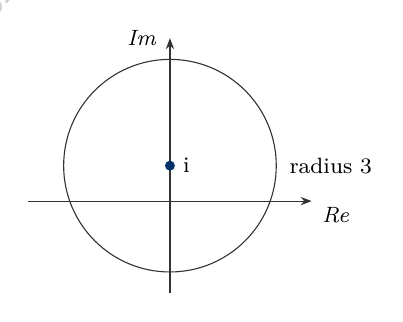
\begin{tikzpicture}[line join=round]
\draw[-{Stealth[length=4pt]},black!80] (0.432,-2.502) -- (4.032,-2.502);
\node[anchor=west,fill=white,fill opacity=0.85,text opacity=1,inner sep=1pt,font=\footnotesize] at (4.122,-2.682) {\textit{Re}};
\draw[-{Stealth[length=4pt]},black!80] (2.232,-3.672) -- (2.232,-0.432);
\node[anchor=east,fill=white,fill opacity=0.85,text opacity=1,inner sep=1pt,font=\footnotesize] at (2.106,-0.432) {\textit{Im}};
\draw[black!80] (2.232,-2.052) circle (1.350);
\fill[FAUblue] (2.232,-2.052) circle (0.063);
\node[anchor=west,fill=white,fill opacity=0.85,text opacity=1,inner sep=1pt,font=\footnotesize] at (2.358,-2.052) {i};
\node[anchor=west,fill=white,fill opacity=0.85,text opacity=1,inner sep=1pt,font=\footnotesize] at (3.708,-2.052) {radius 3};
\end{tikzpicture}\par\smallskip{\small\raggedright \textbf{\{|\textit{z} \ensuremath{-} i| = 3\}.} The circle with centre i and radius 3; it crosses the imaginary axis at 4i and \ensuremath{-}2i.\par}\end{minipage}
\end{center}
\item Check: 4i and \ensuremath{-}2i are both 3 away from i.
\end{enumerate}
\end{workedbox}

\end{keepsection}
\begin{keepsection}\subsection{Exercise 5.4: Complex polar coordinates}

\begin{workedbox}{4ii \ensuremath{\cdot} Sketch \{\textit{z} \ensuremath{\in} \ensuremath{\mathbb{C}} : |\textit{z}| \ensuremath{-} \textit{z̅} = 1 + 2i\}}
\Needspace{8\baselineskip}
\begin{enumerate}
\item \Needspace{4\baselineskip}
With \textit{z} = \textit{x} + iy: |\textit{z}| \ensuremath{-} \textit{z̅} = \ensuremath{\sqrt{{x}^{2}\, +\, {y}^{2}}} \ensuremath{-} \textit{x} + iy. Comparing with 1 + 2i:

\begin{equation*}{y}\, =\, 2\, \text{and}\, \sqrt{{x}^{2}\, +\, {y}^{2}}\, -\, {x}\, =\, 1\end{equation*}
\item So \ensuremath{\sqrt{{x}^{2}\, +\, 4}} = \textit{x} + 1. A square root is never negative, so \textit{x} + 1 \ensuremath{\geq} 0. Squaring: \textit{x}\textsuperscript{2} + 4 = \textit{x}\textsuperscript{2} + 2x + 1, so 2x = 3 and \textit{x} = {\small\ensuremath{\dfrac{3}{2}}}, which satisfies \textit{x} + 1 \ensuremath{\geq} 0.
\item \Needspace{4\baselineskip}
The set is the single point \textit{z} = {\small\ensuremath{\dfrac{3}{2}}} + 2i.

\Needspace{7\baselineskip}
Check: |{\small\ensuremath{\dfrac{3}{2}}} + 2i| = \ensuremath{\sqrt{\dfrac{9}{4}\, +\, 4}} = {\small\ensuremath{\dfrac{5}{2}}}, and {\small\ensuremath{\dfrac{5}{2}}} \ensuremath{-} ({\small\ensuremath{\dfrac{3}{2}}} \ensuremath{-} 2i) = 1 + 2i.

\Needspace{14\baselineskip}
\begin{center}
\begin{minipage}[t]{0.950\linewidth}\centering
\begin{tikzpicture}[line join=round]
\draw[-{Stealth[length=4pt]},black!80] (0.432,-2.700) -- (3.672,-2.700);
\node[anchor=west,fill=white,fill opacity=0.85,text opacity=1,inner sep=1pt,font=\footnotesize] at (3.762,-2.880) {\textit{Re}};
\draw[-{Stealth[length=4pt]},black!80] (1.242,-3.186) -- (1.242,-0.432);
\node[anchor=east,fill=white,fill opacity=0.85,text opacity=1,inner sep=1pt,font=\footnotesize] at (1.116,-0.432) {\textit{Im}};
\fill[FAUblue] (2.457,-1.080) circle (0.063);
\node[anchor=west,fill=white,fill opacity=0.85,text opacity=1,inner sep=1pt,font=\footnotesize] at (2.583,-1.080) {3/2 + 2i};
\end{tikzpicture}\par\smallskip{\small\raggedright \textbf{\{|\textit{z}| \ensuremath{-} \textit{z̅} = 1 + 2i\}.} Only one point solves the equation: \textit{z} = {\small\ensuremath{\dfrac{3}{2}}} + 2i.\par}\end{minipage}
\end{center}
\end{enumerate}
\end{workedbox}

\end{keepsection}
\begin{keepsection}\subsection{Exercise 5.4: Complex polar coordinates}

\begin{workedbox}{4iii \ensuremath{\cdot} Sketch \{\textit{z} \ensuremath{\in} \ensuremath{\mathbb{C}} : Re({\small\ensuremath{\dfrac{1}{{z}}}}) \ensuremath{\leq} 2\}}
\Needspace{12\baselineskip}
\begin{enumerate}
\item The set needs \textit{z} \ensuremath{\neq} 0. With \textit{z} = \textit{x} + iy, {\small\ensuremath{\dfrac{1}{{z}}}} = {\small\ensuremath{\dfrac{{x}\, -\, \text{iy}}{{x}^{2}\, +\, {y}^{2}}}}, so Re {\small\ensuremath{\dfrac{1}{{z}}}} = {\small\ensuremath{\dfrac{{x}}{{x}^{2}\, +\, {y}^{2}}}}.
\item \Needspace{4\baselineskip}
Multiply by \textit{x}\textsuperscript{2} + \textit{y}\textsuperscript{2} \ensuremath{>} 0 (the direction of \ensuremath{\leq} stays) and complete the square:

\begin{equation*}{x}\, \leq \, 2({x}^{2}\, +\, {y}^{2})\, \Leftrightarrow \, {x}^{2}\, -\, \dfrac{{x}}{2}\, +\, {y}^{2}\, \geq \, 0\, \Leftrightarrow \, \left({x}\, -\, \dfrac{1}{4}\right)^{2}\, +\, {y}^{2}\, \geq \, \dfrac{1}{16}\end{equation*}
\item \Needspace{9\baselineskip}
So the set is everything on or outside the circle with centre {\small\ensuremath{\dfrac{1}{4}}} and radius {\small\ensuremath{\dfrac{1}{4}}}, except the origin, which lies on that circle but is not allowed.

\Needspace{14\baselineskip}
\begin{center}
\begin{minipage}[t]{0.950\linewidth}\centering
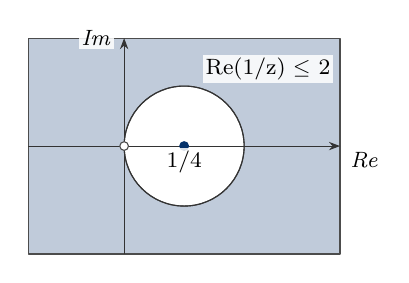
\begin{tikzpicture}[line join=round]
\filldraw[draw=black!70,fill=FAUblue!25] (0.432,-3.174) rectangle (4.392,-0.432);
\draw[draw=black!70,fill=white] (2.412,-1.803) circle (0.762);
\draw[black!80] (2.412,-1.803) circle (0.762);
\draw[-{Stealth[length=4pt]},black!80] (0.432,-1.803) -- (4.392,-1.803);
\node[anchor=west,fill=white,fill opacity=0.85,text opacity=1,inner sep=1pt,font=\footnotesize] at (4.482,-1.983) {\textit{Re}};
\draw[-{Stealth[length=4pt]},black!80] (1.650,-3.174) -- (1.650,-0.432);
\node[anchor=east,fill=white,fill opacity=0.85,text opacity=1,inner sep=1pt,font=\footnotesize] at (1.524,-0.432) {\textit{Im}};
\draw[draw=black!70,fill=white] (1.650,-1.803) circle (0.055);
\fill[FAUblue] (2.412,-1.803) circle (0.063);
\node[fill=white,fill opacity=0.85,text opacity=1,inner sep=1pt,font=\footnotesize] at (2.412,-2.001) {1/4};
\node[fill=white,fill opacity=0.85,text opacity=1,inner sep=1pt,font=\footnotesize] at (3.478,-0.828) {Re(1/z) \ensuremath{\leq} 2};
\end{tikzpicture}\par\smallskip{\small\raggedright \textbf{\{Re({\small\ensuremath{\dfrac{1}{{z}}}}) \ensuremath{\leq} 2\}.} The shaded plane outside the disc of radius {\small\ensuremath{\dfrac{1}{4}}} about {\small\ensuremath{\dfrac{1}{4}}}, with the circle itself included and the origin (the open dot) removed.\par}\end{minipage}
\end{center}
\item Check: \textit{z} = {\small\ensuremath{\dfrac{1}{4}}} is inside the disc and gives Re {\small\ensuremath{\dfrac{1}{{z}}}} = 4 \ensuremath{>} 2 (excluded); \textit{z} = 1 gives 1 \ensuremath{\leq} 2 (included).
\end{enumerate}
\end{workedbox}

\end{keepsection}
\begin{keepsection}\subsection{Self-Study 5.5: Polynomial division and factorisation}

\begin{workedbox}{5a \ensuremath{\cdot} Factorise \textit{x}\textsuperscript{3} \ensuremath{-} 2x\textsuperscript{2} \ensuremath{-} \textit{x} + 2}
\Needspace{7\baselineskip}
\begin{enumerate}
\item \textit{x} = 1 gives 1 \ensuremath{-} 2 \ensuremath{-} 1 + 2 = 0, so (\textit{x} \ensuremath{-} 1) is a factor.
\item \Needspace{5\baselineskip}
Divide: \textit{x}\textsuperscript{3} \ensuremath{-} 2x\textsuperscript{2} \ensuremath{-} \textit{x} + 2 = (\textit{x} \ensuremath{-} 1)(\textit{x}\textsuperscript{2} \ensuremath{-} \textit{x} \ensuremath{-} 2). The quadratic has the roots 2 and \ensuremath{-}1 (product \ensuremath{-}2, sum 1).

\begin{equation*}{x}^{3}\, -\, 2\mathrm{x}^{2}\, -\, {x}\, +\, 2\, =\, ({x}\, -\, 1)({x}\, -\, 2)({x}\, +\, 1)\end{equation*}
\item Check: (\textit{x} \ensuremath{-} 2)(\textit{x} + 1) = \textit{x}\textsuperscript{2} \ensuremath{-} \textit{x} \ensuremath{-} 2, and multiplying by \textit{x} \ensuremath{-} 1 gives back the cubic. The product of the roots, 1 \ensuremath{\cdot} 2 \ensuremath{\cdot} (\ensuremath{-}1) = \ensuremath{-}2, equals minus the constant term, as it must for a monic cubic.
\end{enumerate}
\end{workedbox}

\end{keepsection}
\begin{keepsection}\subsection{Self-Study 5.5: Polynomial division and factorisation}

\begin{workedbox}{5b \ensuremath{\cdot} Factorise \textit{x}\textsuperscript{3} + \textit{x}\textsuperscript{2} \ensuremath{-} 2}
\Needspace{7\baselineskip}
\begin{enumerate}
\item \textit{x} = 1 gives 1 + 1 \ensuremath{-} 2 = 0. Dividing: \textit{x}\textsuperscript{3} + \textit{x}\textsuperscript{2} \ensuremath{-} 2 = (\textit{x} \ensuremath{-} 1)(\textit{x}\textsuperscript{2} + 2x + 2).
\item \Needspace{5\baselineskip}
The quadratic has discriminant 4 \ensuremath{-} 8 = \ensuremath{-}4 \ensuremath{<} 0, so it has no real roots; its complex roots are {\small\ensuremath{\dfrac{-2\, \pm \, 2\mathrm{i}}{2}}} = \ensuremath{-}1 \ensuremath{\pm} i.

\begin{equation*}{x}^{3}\, +\, {x}^{2}\, -\, 2\, =\, ({x}\, -\, 1)({x}^{2}\, +\, 2\mathrm{x}\, +\, 2)\, =\, ({x}\, -\, 1)({x}\, +\, 1\, -\, \mathrm{i})({x}\, +\, 1\, +\, \mathrm{i})\end{equation*}
\item Check: (\textit{x} \ensuremath{-} 1)(\textit{x}\textsuperscript{2} + 2x + 2) = \textit{x}\textsuperscript{3} + 2x\textsuperscript{2} + 2x \ensuremath{-} \textit{x}\textsuperscript{2} \ensuremath{-} 2x \ensuremath{-} 2 = \textit{x}\textsuperscript{3} + \textit{x}\textsuperscript{2} \ensuremath{-} 2. Over \ensuremath{\mathbb{R}} the factorisation stops at the quadratic; the complex pair is conjugate, as for every real polynomial.
\end{enumerate}
\end{workedbox}

\end{keepsection}
\begin{keepsection}\subsection{Self-Study 5.5: Polynomial division and factorisation}

\begin{workedbox}{5c \ensuremath{\cdot} Factorise \textit{x}\textsuperscript{4} \ensuremath{-} 5x\textsuperscript{2} + 4}
\Needspace{7\baselineskip}
\begin{enumerate}
\item \textit{x} = 1: 1 \ensuremath{-} 5 + 4 = 0. Dividing by \textit{x} \ensuremath{-} 1 gives \textit{x}\textsuperscript{3} + \textit{x}\textsuperscript{2} \ensuremath{-} 4x \ensuremath{-} 4.
\item \Needspace{5\baselineskip}
\textit{x} = \ensuremath{-}1 is a root of that cubic: \ensuremath{-}1 + 1 + 4 \ensuremath{-} 4 = 0. Dividing by \textit{x} + 1 gives \textit{x}\textsuperscript{2} \ensuremath{-} 4 = (\textit{x} \ensuremath{-} 2)(\textit{x} + 2).

\begin{equation*}{x}^{4}\, -\, 5\mathrm{x}^{2}\, +\, 4\, =\, ({x}\, -\, 1)({x}\, +\, 1)({x}\, -\, 2)({x}\, +\, 2)\end{equation*}
\item Check with \textit{u} = \textit{x}\textsuperscript{2}: \textit{u}\textsuperscript{2} \ensuremath{-} 5u + 4 = (\textit{u} \ensuremath{-} 1)(\textit{u} \ensuremath{-} 4), and \textit{u} \ensuremath{-} 1 = (\textit{x} \ensuremath{-} 1)(\textit{x} + 1), \textit{u} \ensuremath{-} 4 = (\textit{x} \ensuremath{-} 2)(\textit{x} + 2).
\end{enumerate}
\end{workedbox}

\end{keepsection}
\begin{keepsection}\subsection{Self-Study 5.5: Polynomial division and factorisation}

\begin{workedbox}{5d \ensuremath{\cdot} Divide 2x\textsuperscript{3} + 3x\textsuperscript{2} \ensuremath{-} 5x + 1 by \textit{x}\textsuperscript{2} + \textit{x} \ensuremath{-} 1 with remainder}
\Needspace{7\baselineskip}
\begin{enumerate}
\item First term 2x: 2x(\textit{x}\textsuperscript{2} + \textit{x} \ensuremath{-} 1) = 2x\textsuperscript{3} + 2x\textsuperscript{2} \ensuremath{-} 2x. Subtracting leaves \textit{x}\textsuperscript{2} \ensuremath{-} 3x + 1.
\item \Needspace{5\baselineskip}
Next term 1: \textit{x}\textsuperscript{2} + \textit{x} \ensuremath{-} 1. Subtracting leaves \ensuremath{-}4x + 2, whose degree is below 2, so the division stops.

\begin{equation*}2\mathrm{x}^{3}\, +\, 3\mathrm{x}^{2}\, -\, 5\mathrm{x}\, +\, 1\, =\, (2\mathrm{x}\, +\, 1)({x}^{2}\, +\, {x}\, -\, 1)\, +\, (-4\mathrm{x}\, +\, 2)\end{equation*}
\item Quotient 2x + 1, remainder \ensuremath{-}4x + 2. Check: (2x + 1)(\textit{x}\textsuperscript{2} + \textit{x} \ensuremath{-} 1) = 2x\textsuperscript{3} + 3x\textsuperscript{2} \ensuremath{-} \textit{x} \ensuremath{-} 1, and adding \ensuremath{-}4x + 2 gives 2x\textsuperscript{3} + 3x\textsuperscript{2} \ensuremath{-} 5x + 1.
\end{enumerate}
\end{workedbox}

\end{keepsection}
\begin{keepsection}\subsection{Self-Study 5.6: Roots of polynomials}

\begin{workedbox}{6a \ensuremath{\cdot} Show deg(\textit{P} \ensuremath{\cdot} \textit{Q}) = deg \textit{P} + deg \textit{Q}}
\Needspace{8\baselineskip}
\begin{enumerate}
\item Multiplying out, every term of \textit{P} \ensuremath{\cdot} \textit{Q} has the form \textit{a}\textsubscript{i}\textit{b}\textsubscript{j}\textit{x}\textsuperscript{i + j} with i \ensuremath{\leq} \textit{n} and j \ensuremath{\leq} \textit{k}, so no power above \textit{x}\textsuperscript{\textit{n} + \textit{k}} appears.
\item \Needspace{5\baselineskip}
The power \textit{x}\textsuperscript{\textit{n} + \textit{k}} arises only from i = \textit{n}, j = \textit{k}, with coefficient \textit{a}\textsubscript{\textit{n}}\textit{b}\textsubscript{\textit{k}}. In \ensuremath{\mathbb{R}} a product of two nonzero numbers is nonzero, so \textit{a}\textsubscript{\textit{n}}\textit{b}\textsubscript{\textit{k}} \ensuremath{\neq} 0.

\begin{equation*}{P}({x}){Q}({x})\, =\, {a}_{{n}}{b}_{{k}}{x}^{{n}\, +\, {k}}\, +\, (\text{lower}\, \text{powers}),\, {a}_{{n}}{b}_{{k}}\, ≠\, 0\end{equation*}
\item Hence deg(\textit{P} \ensuremath{\cdot} \textit{Q}) = \textit{n} + \textit{k} = deg \textit{P} + deg \textit{Q}. The step that matters is \textit{a}\textsubscript{\textit{n}}\textit{b}\textsubscript{\textit{k}} \ensuremath{\neq} 0: without it the top terms could cancel.
\end{enumerate}
\end{workedbox}

\end{keepsection}
\begin{keepsection}\subsection{Self-Study 5.6: Roots of polynomials}

\begin{workedbox}{6b \ensuremath{\cdot} Show \textit{x}\textsuperscript{\textit{k}} \ensuremath{-} \textit{x}\textsubscript{0}\textsuperscript{\textit{k}} = (\textit{x} \ensuremath{-} \textit{x}\textsubscript{0}) \ensuremath{\textstyle\sum} \textit{x}\textsuperscript{\textit{k}\ensuremath{-}1\ensuremath{-}j}\textit{x}\textsubscript{0}\textsuperscript{j}}
\Needspace{8\baselineskip}
\begin{enumerate}
\item \Needspace{4\baselineskip}
Multiply the sum by \textit{x} and by \ensuremath{-}\textit{x}\textsubscript{0} separately:

\begin{equation*}({x}\, -\, {x}_{0})\sum_{\mathrm{j}=0}^{{k}-1} \, {x}^{{k}-1-\mathrm{j}}{x}_{0}^{\mathrm{j}}\, =\, \sum_{\mathrm{j}=0}^{{k}-1} \, {x}^{{k}-\mathrm{j}}{x}_{0}^{\mathrm{j}}\, -\, \sum_{\mathrm{j}=0}^{{k}-1} \, {x}^{{k}-1-\mathrm{j}}{x}_{0}^{\mathrm{j}+1}\end{equation*}
\item \Needspace{6\baselineskip}
Shift the index in the second sum (j + 1 \ensuremath{\to} j), so it runs over j = 1, …, \textit{k} with terms \textit{x}\textsuperscript{\textit{k}\ensuremath{-}j}\textit{x}\textsubscript{0}\textsuperscript{j}. All terms with j = 1, …, \textit{k} \ensuremath{-} 1 cancel; only j = 0 from the first sum and j = \textit{k} from the second remain:

\begin{equation*}=\, {x}^{{k}}\, -\, {x}_{0}^{{k}}\end{equation*}
\item Check with \textit{k} = 2: (\textit{x} \ensuremath{-} \textit{x}\textsubscript{0})(\textit{x} + \textit{x}\textsubscript{0}) = \textit{x}\textsuperscript{2} \ensuremath{-} \textit{x}\textsubscript{0}\textsuperscript{2}.
\end{enumerate}
\end{workedbox}

\end{keepsection}
\begin{keepsection}\subsection{Self-Study 5.6: Roots of polynomials}

\begin{workedbox}{6c \ensuremath{\cdot} Show \textit{P}(\textit{x}) = (\textit{x} \ensuremath{-} \textit{x}\textsubscript{0})\textit{Q}(\textit{x}) with deg \textit{Q} = \textit{n} \ensuremath{-} 1}
\Needspace{7\baselineskip}
\begin{enumerate}
\item \Needspace{4\baselineskip}
Since \textit{P}(\textit{x}\textsubscript{0}) = 0, \textit{P}(\textit{x}) = \textit{P}(\textit{x}) \ensuremath{-} \textit{P}(\textit{x}\textsubscript{0}). The constant \textit{a}\textsubscript{0} cancels:

\begin{equation*}{P}({x})\, =\, \sum_{{k}=1}^{{n}} \, {a}_{{k}}({x}^{{k}}\, -\, {x}_{0}^{{k}})\end{equation*}
\item \Needspace{4\baselineskip}
Apply 6b to every term and pull out the common factor:

\begin{equation*}{P}({x})\, =\, ({x}\, -\, {x}_{0})\, \sum_{{k}=1}^{{n}} \, {a}_{{k}}\, \sum_{\mathrm{j}=0}^{{k}-1} \, {x}^{{k}-1-\mathrm{j}}{x}_{0}^{\mathrm{j}}\, =:\, ({x}\, -\, {x}_{0}){Q}({x})\end{equation*}
\item \textit{Q} is a polynomial. Its highest power \textit{x}\textsuperscript{\textit{n}\ensuremath{-}1} comes only from \textit{k} = \textit{n}, j = 0, with coefficient \textit{a}\textsubscript{\textit{n}} \ensuremath{\neq} 0, so deg \textit{Q} = \textit{n} \ensuremath{-} 1 (consistent with 6a: 1 + (\textit{n} \ensuremath{-} 1) = \textit{n}).
\end{enumerate}
\end{workedbox}

\end{keepsection}
\begin{keepsection}\subsection{Self-Study 5.6: Roots of polynomials}

\begin{workedbox}{6d \ensuremath{\cdot} Prove Theorem 3.7 by induction on \textit{n}}
\Needspace{10\baselineskip}
\begin{enumerate}
\item \textbf{Claim A(\textit{n}):} every real polynomial of degree \textit{n} has at most \textit{n} real roots.
\item \textbf{Base case \textit{n} = 1:} \textit{a}\textsubscript{1}\textit{x} + \textit{a}\textsubscript{0} with \textit{a}\textsubscript{1} \ensuremath{\neq} 0 has exactly one root, \textit{x} = \ensuremath{-}{\small\ensuremath{\dfrac{{a}_{0}}{{a}_{1}}}}.
\item \textbf{Induction step:} assume A(\textit{n}) and let \textit{P} have degree \textit{n} + 1. If \textit{P} has no real root, there is nothing to show. Otherwise pick a root \textit{x}\textsubscript{0}; by 6c, \textit{P}(\textit{x}) = (\textit{x} \ensuremath{-} \textit{x}\textsubscript{0})\textit{Q}(\textit{x}) with deg \textit{Q} = \textit{n}.
\item \Needspace{6\baselineskip}
If \textit{P}(\textit{x}) = 0 then \textit{x} \ensuremath{-} \textit{x}\textsubscript{0} = 0 or \textit{Q}(\textit{x}) = 0, because a product of real numbers is zero only when a factor is. So every root of \textit{P} is \textit{x}\textsubscript{0} or a root of \textit{Q}, and by A(\textit{n}) \textit{Q} has at most \textit{n} real roots. Hence \textit{P} has at most \textit{n} + 1.

Therefore A(\textit{n}) holds for all \textit{n} \ensuremath{\in} \ensuremath{\mathbb{N}}.
\end{enumerate}
\end{workedbox}

\end{keepsection}
\begin{keepsection}\subsection{Self-Study 5.7: Difference formulas}

\begin{workedbox}{7a \ensuremath{\cdot} Prove the difference formulas for sine and cosine}
\Needspace{10\baselineskip}
\begin{enumerate}
\item Let \textit{a} = {\small\ensuremath{\dfrac{{x}\, +\, {y}}{2}}} and \textit{b} = {\small\ensuremath{\dfrac{{x}\, -\, {y}}{2}}}. Then \textit{x} = \textit{a} + b and \textit{y} = \textit{a} \ensuremath{-} b.
\item \Needspace{5\baselineskip}
Sine: by the addition theorems, sin(\textit{a} + \textit{b}) \ensuremath{-} sin(\textit{a} \ensuremath{-} \textit{b}) = (sin a cos \textit{b} + cos a sin \textit{b}) \ensuremath{-} (sin a cos \textit{b} \ensuremath{-} cos a sin \textit{b}) = 2 cos a sin b.

\begin{equation*}\sin \, {x}\, -\, \sin \, {y}\, =\, 2\, \cos \left(\dfrac{{x}\, +\, {y}}{2}\right)\, \sin \left(\dfrac{{x}\, -\, {y}}{2}\right)\end{equation*}
\item \Needspace{5\baselineskip}
Cosine: cos(\textit{a} + \textit{b}) \ensuremath{-} cos(\textit{a} \ensuremath{-} \textit{b}) = (cos a cos \textit{b} \ensuremath{-} sin a sin \textit{b}) \ensuremath{-} (cos a cos \textit{b} + sin a sin \textit{b}) = \ensuremath{-}2 sin a sin b. Since sine is odd, \ensuremath{-}sin \textit{b} = sin(\ensuremath{-}\textit{b}) = sin {\small\ensuremath{\dfrac{{y}\, -\, {x}}{2}}}:

\begin{equation*}\cos \, {x}\, -\, \cos \, {y}\, =\, 2\, \sin \left(\dfrac{{x}\, +\, {y}}{2}\right)\, \sin \left(\dfrac{{y}\, -\, {x}}{2}\right)\end{equation*}
\item Check with \textit{x} = {\small\ensuremath{\dfrac{π}{2}}}, \textit{y} = 0: sin {\small\ensuremath{\dfrac{π}{2}}} \ensuremath{-} 0 = 1, and 2 cos {\small\ensuremath{\dfrac{π}{4}}} sin {\small\ensuremath{\dfrac{π}{4}}} = 2 \ensuremath{\cdot} {\small\ensuremath{\dfrac{\sqrt{2}}{2}}} \ensuremath{\cdot} {\small\ensuremath{\dfrac{\sqrt{2}}{2}}} = 1.
\end{enumerate}
\end{workedbox}

\end{keepsection}
\begin{keepsection}\subsection{Self-Study 5.7: Difference formulas}

\begin{workedbox}{7b \ensuremath{\cdot} Show sin \textit{x} \ensuremath{-} sin(\textit{x} \ensuremath{-} {\small\ensuremath{\dfrac{π}{3}}}) = cos(\textit{x} \ensuremath{-} {\small\ensuremath{\dfrac{π}{6}}}) and cos \textit{x} \ensuremath{-} cos(\textit{x} + {\small\ensuremath{\dfrac{π}{3}}}) = sin(\textit{x} + {\small\ensuremath{\dfrac{π}{6}}})}
\Needspace{6\baselineskip}
\begin{enumerate}
\item With \textit{y} = \textit{x} \ensuremath{-} {\small\ensuremath{\dfrac{π}{3}}}: {\small\ensuremath{\dfrac{{x}\, +\, {y}}{2}}} = \textit{x} \ensuremath{-} {\small\ensuremath{\dfrac{π}{6}}} and {\small\ensuremath{\dfrac{{x}\, -\, {y}}{2}}} = {\small\ensuremath{\dfrac{π}{6}}}. So sin \textit{x} \ensuremath{-} sin(\textit{x} \ensuremath{-} {\small\ensuremath{\dfrac{π}{3}}}) = 2 cos(\textit{x} \ensuremath{-} {\small\ensuremath{\dfrac{π}{6}}}) sin {\small\ensuremath{\dfrac{π}{6}}} = 2 \ensuremath{\cdot} \ensuremath{\tfrac12} \ensuremath{\cdot} cos(\textit{x} \ensuremath{-} {\small\ensuremath{\dfrac{π}{6}}}) = cos(\textit{x} \ensuremath{-} {\small\ensuremath{\dfrac{π}{6}}}).
\item \Needspace{5\baselineskip}
With \textit{y} = \textit{x} + {\small\ensuremath{\dfrac{π}{3}}}: {\small\ensuremath{\dfrac{{x}\, +\, {y}}{2}}} = \textit{x} + {\small\ensuremath{\dfrac{π}{6}}} and {\small\ensuremath{\dfrac{{y}\, -\, {x}}{2}}} = {\small\ensuremath{\dfrac{π}{6}}}. So cos \textit{x} \ensuremath{-} cos(\textit{x} + {\small\ensuremath{\dfrac{π}{3}}}) = 2 sin(\textit{x} + {\small\ensuremath{\dfrac{π}{6}}}) sin {\small\ensuremath{\dfrac{π}{6}}} = sin(\textit{x} + {\small\ensuremath{\dfrac{π}{6}}}).

Check with \textit{x} = 0: 0 \ensuremath{-} sin(\ensuremath{-}{\small\ensuremath{\dfrac{π}{3}}}) = {\small\ensuremath{\dfrac{\sqrt{3}}{2}}} = cos(\ensuremath{-}{\small\ensuremath{\dfrac{π}{6}}}), and 1 \ensuremath{-} cos {\small\ensuremath{\dfrac{π}{3}}} = \ensuremath{\tfrac12} = sin {\small\ensuremath{\dfrac{π}{6}}}.
\end{enumerate}
\end{workedbox}

\end{keepsection}
\begin{keepsection}\subsection{Self-Study 5.7: Difference formulas}

\begin{workedbox}{7c-i \ensuremath{\cdot} Solve sin \textit{x} \ensuremath{-} sin(\textit{x} \ensuremath{-} {\small\ensuremath{\dfrac{π}{3}}}) = \ensuremath{\tfrac12} for \textit{x} \ensuremath{\in} [π, 2π]}
\Needspace{8\baselineskip}
\begin{enumerate}
\item By 7b the equation reads cos \textit{t} = \ensuremath{\tfrac12} with \textit{t} = \textit{x} \ensuremath{-} {\small\ensuremath{\dfrac{π}{6}}}. For \textit{x} \ensuremath{\in} [π, 2π], \textit{t} runs through [{\small\ensuremath{\dfrac{5π}{6}}}, {\small\ensuremath{\dfrac{11π}{6}}}].
\item arccos \ensuremath{\tfrac12} = {\small\ensuremath{\dfrac{π}{3}}}, but {\small\ensuremath{\dfrac{π}{3}}} is not in that range. Using cos \textit{t} = cos(2π \ensuremath{-} \textit{t}), the other angle with cosine \ensuremath{\tfrac12} is 2π \ensuremath{-} {\small\ensuremath{\dfrac{π}{3}}} = {\small\ensuremath{\dfrac{5π}{3}}}, which is in the range.
\item \Needspace{4\baselineskip}
So \textit{t} = {\small\ensuremath{\dfrac{5π}{3}}} and \textit{x} = {\small\ensuremath{\dfrac{5π}{3}}} + {\small\ensuremath{\dfrac{π}{6}}} = {\small\ensuremath{\dfrac{11π}{6}}}. No other angle in [{\small\ensuremath{\dfrac{5π}{6}}}, {\small\ensuremath{\dfrac{11π}{6}}}] has cosine \ensuremath{\tfrac12}.

Check: sin {\small\ensuremath{\dfrac{11π}{6}}} \ensuremath{-} sin {\small\ensuremath{\dfrac{3π}{2}}} = \ensuremath{-}\ensuremath{\tfrac12} \ensuremath{-} (\ensuremath{-}1) = \ensuremath{\tfrac12}.
\end{enumerate}
\end{workedbox}

\end{keepsection}
\begin{keepsection}\subsection{Self-Study 5.7: Difference formulas}

\begin{workedbox}{7c-ii \ensuremath{\cdot} Solve cos \textit{x} \ensuremath{-} cos(\textit{x} + {\small\ensuremath{\dfrac{π}{3}}}) = \ensuremath{-}{\small\ensuremath{\dfrac{\sqrt{2}}{2}}} for \textit{x} \ensuremath{\in} [{\small\ensuremath{\dfrac{π}{2}}}, {\small\ensuremath{\dfrac{3π}{2}}}]}
\Needspace{8\baselineskip}
\begin{enumerate}
\item By 7b the equation reads sin \textit{t} = \ensuremath{-}{\small\ensuremath{\dfrac{\sqrt{2}}{2}}} with \textit{t} = \textit{x} + {\small\ensuremath{\dfrac{π}{6}}}. For \textit{x} \ensuremath{\in} [{\small\ensuremath{\dfrac{π}{2}}}, {\small\ensuremath{\dfrac{3π}{2}}}], \textit{t} runs through [{\small\ensuremath{\dfrac{2π}{3}}}, {\small\ensuremath{\dfrac{5π}{3}}}].
\item arcsin(\ensuremath{-}{\small\ensuremath{\dfrac{\sqrt{2}}{2}}}) = \ensuremath{-}{\small\ensuremath{\dfrac{π}{4}}}, which is not in that range. Using sin \textit{t} = sin(π \ensuremath{-} \textit{t}), the angle π \ensuremath{-} (\ensuremath{-}{\small\ensuremath{\dfrac{π}{4}}}) = {\small\ensuremath{\dfrac{5π}{4}}} also has sine \ensuremath{-}{\small\ensuremath{\dfrac{\sqrt{2}}{2}}}, and it is in the range. The next candidate, {\small\ensuremath{\dfrac{7π}{4}}}, is above {\small\ensuremath{\dfrac{5π}{3}}}.
\item \Needspace{4\baselineskip}
So \textit{t} = {\small\ensuremath{\dfrac{5π}{4}}} and \textit{x} = {\small\ensuremath{\dfrac{5π}{4}}} \ensuremath{-} {\small\ensuremath{\dfrac{π}{6}}} = {\small\ensuremath{\dfrac{13π}{12}}}.

Check numerically: cos({\small\ensuremath{\dfrac{13π}{12}}}) \ensuremath{-} cos({\small\ensuremath{\dfrac{17π}{12}}}) \ensuremath{\approx} \ensuremath{-}0.966 \ensuremath{-} (\ensuremath{-}0.259) = \ensuremath{-}0.707 \ensuremath{\approx} \ensuremath{-}{\small\ensuremath{\dfrac{\sqrt{2}}{2}}}.
\end{enumerate}
\end{workedbox}

\end{keepsection}
\begin{keepsection}\subsection{Self-Study 5.8: Polar coordinates}

\begin{workedbox}{8a \ensuremath{\cdot} Polar coordinates of (\ensuremath{-}\ensuremath{\sqrt{3}}, 1) and (\ensuremath{\sqrt{2}}, \ensuremath{-}5)}
\Needspace{7\baselineskip}
\begin{enumerate}
\item \textbf{(\ensuremath{-}\ensuremath{\sqrt{3}}, 1):} \textit{r} = \ensuremath{\sqrt{3\, +\, 1}} = 2. Quadrant II, and arctan({\small\ensuremath{\dfrac{1}{-\sqrt{3}}}}) = \ensuremath{-}{\small\ensuremath{\dfrac{π}{6}}}, so φ = \ensuremath{-}{\small\ensuremath{\dfrac{π}{6}}} + π = {\small\ensuremath{\dfrac{5π}{6}}}.
\item \Needspace{4\baselineskip}
\textbf{(\ensuremath{\sqrt{2}}, \ensuremath{-}5):} \textit{r} = \ensuremath{\sqrt{2\, +\, 25}} = \ensuremath{\sqrt{27}} = 3\ensuremath{\sqrt{3}} \ensuremath{\approx} 5.20. Quadrant IV (\textit{x} \ensuremath{>} 0, \textit{y} \ensuremath{<} 0), so add 2π:

\begin{equation*}φ\, =\, 2π\, -\, \arctan \left(\dfrac{5}{\sqrt{2}}\right)\, \approx \, 4.99\end{equation*}
\item Results: (2, {\small\ensuremath{\dfrac{5π}{6}}}) and (3\ensuremath{\sqrt{3}}, 2π \ensuremath{-} arctan {\small\ensuremath{\dfrac{5}{\sqrt{2}}}}) \ensuremath{\approx} (5.20, 4.99). Check: 2 cos {\small\ensuremath{\dfrac{5π}{6}}} = \ensuremath{-}\ensuremath{\sqrt{3}} and 2 sin {\small\ensuremath{\dfrac{5π}{6}}} = 1.
\end{enumerate}
\end{workedbox}

\end{keepsection}
\begin{keepsection}\subsection{Self-Study 5.8: Polar coordinates}

\begin{workedbox}{8b \ensuremath{\cdot} Describe the sketched ring section in Cartesian and polar coordinates}
\Needspace{14\baselineskip}
\begin{enumerate}
\item \textbf{Reading the sketch:} the inner boundary meets the negative \textit{x}-axis at \ensuremath{-}\ensuremath{\sqrt{2}}, so the inner radius is \ensuremath{\sqrt{2}}. The outer corner on the dashed line is (2, 2), at distance \ensuremath{\sqrt{8}} = 2\ensuremath{\sqrt{2}}. The region starts on the dashed line \textit{y} = \textit{x} (angle {\small\ensuremath{\dfrac{π}{4}}}), runs counterclockwise through the left half-plane, and ends on the negative \textit{y}-axis (angle {\small\ensuremath{\dfrac{3π}{2}}}). The boundary belongs to \textit{M}.
\item \Needspace{4\baselineskip}
\textbf{Polar:}

\begin{equation*}{M}\, =\, \{({r},\, φ)\, :\, \sqrt{2}\, \leq \, {r}\, \leq \, 2\sqrt{2},\, \dfrac{π}{4}\, \leq \, φ\, \leq \, \dfrac{3π}{2}\}\end{equation*}
\item \Needspace{5\baselineskip}
\textbf{Cartesian:} the radius condition is 2 \ensuremath{\leq} \textit{x}\textsuperscript{2} + \textit{y}\textsuperscript{2} \ensuremath{\leq} 8. The angles from {\small\ensuremath{\dfrac{π}{4}}} to {\small\ensuremath{\dfrac{3π}{2}}} are the closed left half-plane \textit{x} \ensuremath{\leq} 0 together with the part of the right half-plane on or above \textit{y} = \textit{x}:

\Needspace{8\baselineskip}
\begin{equation*}{M}\, =\, \{({x},\, {y})\, :\, 2\, \leq \, {x}^{2}\, +\, {y}^{2}\, \leq \, 8\, \text{and}\, ({x}\, \leq \, 0\, \text{or}\, {y}\, \geq \, {x})\}\end{equation*}

\Needspace{14\baselineskip}
\begin{center}
\begin{minipage}[t]{0.950\linewidth}\centering
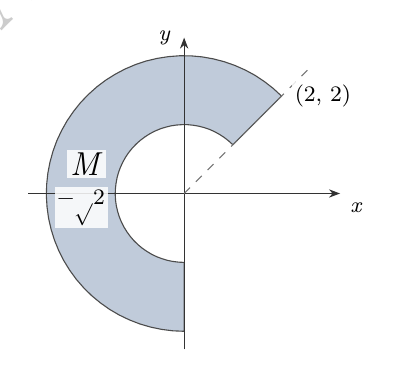
\begin{tikzpicture}[line join=round]
\filldraw[draw=black!70,fill=FAUblue!25] (3.649,-1.175) -- (3.544,-1.078) -- (3.431,-0.990) -- (3.312,-0.911) -- (3.186,-0.843) -- (3.055,-0.785) -- (2.920,-0.738) -- (2.781,-0.702) -- (2.640,-0.677) -- (2.498,-0.664) -- (2.355,-0.663) -- (2.212,-0.674) -- (2.071,-0.696) -- (1.932,-0.729) -- (1.796,-0.774) -- (1.664,-0.830) -- (1.537,-0.897) -- (1.416,-0.973) -- (1.302,-1.059) -- (1.195,-1.155) -- (1.096,-1.258) -- (1.007,-1.370) -- (0.926,-1.488) -- (0.856,-1.612) -- (0.795,-1.742) -- (0.746,-1.877) -- (0.708,-2.015) -- (0.681,-2.155) -- (0.666,-2.298) -- (0.662,-2.441) -- (0.671,-2.584) -- (0.690,-2.725) -- (0.722,-2.865) -- (0.764,-3.001) -- (0.818,-3.134) -- (0.882,-3.262) -- (0.957,-3.384) -- (1.041,-3.500) -- (1.135,-3.608) -- (1.237,-3.709) -- (1.347,-3.800) -- (1.464,-3.883) -- (1.587,-3.955) -- (1.716,-4.017) -- (1.850,-4.069) -- (1.987,-4.109) -- (2.127,-4.138) -- (2.269,-4.156) -- (2.412,-4.162) -- (2.412,-3.287) -- (2.341,-3.284) -- (2.269,-3.275) -- (2.199,-3.261) -- (2.131,-3.240) -- (2.064,-3.215) -- (2.000,-3.184) -- (1.938,-3.147) -- (1.879,-3.106) -- (1.824,-3.060) -- (1.773,-3.010) -- (1.727,-2.956) -- (1.685,-2.898) -- (1.647,-2.837) -- (1.615,-2.773) -- (1.588,-2.707) -- (1.567,-2.638) -- (1.551,-2.569) -- (1.541,-2.498) -- (1.537,-2.426) -- (1.539,-2.355) -- (1.547,-2.284) -- (1.560,-2.213) -- (1.579,-2.144) -- (1.604,-2.077) -- (1.634,-2.012) -- (1.669,-1.950) -- (1.709,-1.891) -- (1.754,-1.835) -- (1.804,-1.783) -- (1.857,-1.736) -- (1.914,-1.693) -- (1.975,-1.654) -- (2.038,-1.621) -- (2.104,-1.593) -- (2.172,-1.571) -- (2.241,-1.554) -- (2.312,-1.543) -- (2.383,-1.538) -- (2.455,-1.538) -- (2.526,-1.545) -- (2.597,-1.557) -- (2.666,-1.575) -- (2.734,-1.598) -- (2.799,-1.627) -- (2.862,-1.662) -- (2.922,-1.701) -- (2.978,-1.745) -- (3.031,-1.793) -- cycle;
\draw[-{Stealth[length=4pt]},black!80] (0.432,-2.412) -- (4.392,-2.412);
\node[anchor=west,fill=white,fill opacity=0.85,text opacity=1,inner sep=1pt,font=\footnotesize] at (4.482,-2.592) {\textit{x}};
\draw[-{Stealth[length=4pt]},black!80] (2.412,-4.392) -- (2.412,-0.432);
\node[anchor=east,fill=white,fill opacity=0.85,text opacity=1,inner sep=1pt,font=\footnotesize] at (2.286,-0.432) {\textit{y}};
\draw[black!55,dashed] (2.412,-2.412) -- (4.021,-0.803);
\node[anchor=east,fill=white,fill opacity=0.85,text opacity=1,inner sep=1pt,font=\footnotesize] at (1.447,-2.592) {\ensuremath{-}\ensuremath{\surd}2};
\node[anchor=west,fill=white,fill opacity=0.85,text opacity=1,inner sep=1pt,font=\footnotesize] at (3.775,-1.174) {(2, 2)};
\node[fill=white,fill opacity=0.85,text opacity=1,inner sep=1pt,font=\large] at (1.174,-2.041) {\textit{M}};
\end{tikzpicture}\par\smallskip{\small\raggedright \textbf{The set \textit{M}.} The ring between radii \ensuremath{\sqrt{2}} and 2\ensuremath{\sqrt{2}}, from the dashed line \textit{y} = \textit{x} counterclockwise to the negative \textit{y}-axis.\par}\end{minipage}
\end{center}
\item Check: (\ensuremath{-}2, 0) has \textit{x}\textsuperscript{2} + \textit{y}\textsuperscript{2} = 4 and \textit{x} \ensuremath{\leq} 0, and angle π, so it is in \textit{M} by both descriptions; (2, 0) has angle 0 and \textit{y} \ensuremath{<} \textit{x}, so it is in neither.
\end{enumerate}
\end{workedbox}

\end{keepsection}
\begin{keepsection}\subsection{Self-Study 5.8: Polar coordinates}

\begin{workedbox}{8c \ensuremath{\cdot} Write \textit{y} = 2x \ensuremath{-} 5 as \textit{r} = \textit{f}(φ) and find where \textit{f}(φ) \ensuremath{>} 0}
\Needspace{10\baselineskip}
\begin{enumerate}
\item \Needspace{4\baselineskip}
Substitute: \textit{r} sin φ = 2r cos φ \ensuremath{-} 5, so \textit{r}(2 cos φ \ensuremath{-} sin φ) = 5 and

\begin{equation*}{r}\, =\, {f}(φ)\, =\, \dfrac{5}{2\, \cos \, φ\, -\, \sin \, φ}\end{equation*}
\item \textit{f}(φ) is defined and positive exactly when 2 cos φ \ensuremath{-} sin φ \ensuremath{>} 0. The denominator is zero where tan φ = 2, that is at φ = arctan 2 \ensuremath{\approx} 0.35π and φ \ensuremath{\approx} 1.35π; between them it is negative (at φ = π it equals \ensuremath{-}2).
\item \Needspace{4\baselineskip}
So, with φ \ensuremath{\in} [0, 2π):

\Needspace{6\baselineskip}
\begin{equation*}{f}(φ)\, >\, 0\, \Leftrightarrow \, φ\, \in \, [0,\, \arctan \, 2)\, \cup \, (\arctan \, 2\, +\, π,\, 2π)\, \approx \, [0,\, 0.35π)\, \cup \, (1.35π,\, 2π)\end{equation*}

Check: φ = 0 gives \textit{r} = {\small\ensuremath{\dfrac{5}{2}}}, the point (2.5, 0), and indeed 2 \ensuremath{\cdot} 2.5 \ensuremath{-} 5 = 0. The line passes below the origin, so the rays that reach it point to the right and downwards, as the angle ranges say.
\end{enumerate}
\end{workedbox}

\end{keepsection}
\begin{keepsection}\subsection{Self-Study 5.9: Arithmetic rules}

\begin{workedbox}{9a \ensuremath{\cdot} Evaluate \ensuremath{\tfrac12} log\textsubscript{2}(4e\textsuperscript{2}) \ensuremath{-} {\small\ensuremath{\dfrac{1}{\ln \, 2}}}}
\Needspace{5\baselineskip}
\begin{enumerate}
\item log\textsubscript{2}(4e\textsuperscript{2}) = log\textsubscript{2} 4 + log\textsubscript{2}(e\textsuperscript{2}) = 2 + 2 log\textsubscript{2} e, and log\textsubscript{2} e = {\small\ensuremath{\dfrac{\ln \, \mathrm{e}}{\ln \, 2}}} = {\small\ensuremath{\dfrac{1}{\ln \, 2}}}.
\item \Needspace{4\baselineskip}
So the expression is

\Needspace{4\baselineskip}
\begin{equation*}\tfrac{1}{2}\left(2\, +\, \dfrac{2}{\ln \, 2}\right)\, -\, \dfrac{1}{\ln \, 2}\, =\, 1\, +\, \dfrac{1}{\ln \, 2}\, -\, \dfrac{1}{\ln \, 2}\, =\, 1\end{equation*}

Check numerically: \ensuremath{\tfrac12} log\textsubscript{2}(29.56) \ensuremath{\approx} 2.443 and {\small\ensuremath{\dfrac{1}{\ln \, 2}}} \ensuremath{\approx} 1.443; their difference is 1.
\end{enumerate}
\end{workedbox}

\end{keepsection}
\begin{keepsection}\subsection{Self-Study 5.9: Arithmetic rules}

\begin{workedbox}{9b \ensuremath{\cdot} Simplify ln(\textit{x}\textsuperscript{2/3}) \ensuremath{-} ln((\textit{x}\textsuperscript{\ensuremath{-}4})\textsuperscript{1/3}) for \textit{x} \ensuremath{>} 0, the second term being the cube root of \textit{x}\textsuperscript{\ensuremath{-}4}}
\Needspace{5\baselineskip}
\begin{enumerate}
\item \Needspace{4\baselineskip}
The cube root is the power \ensuremath{\tfrac13}: (\textit{x}\textsuperscript{\ensuremath{-}4})\textsuperscript{1/3} = \textit{x}\textsuperscript{\ensuremath{-}4/3}. With ln(\textit{x}\textsuperscript{α}) = α ln \textit{x} (Self-Study 5.14):

\begin{equation*}\ln ({x}^{2/3})\, -\, \ln ({x}^{-4/3})\, =\, \dfrac{2}{3}\, \ln \, {x}\, +\, \dfrac{4}{3}\, \ln \, {x}\, =\, 2\, \ln \, {x}\end{equation*}
\item Equivalently ln {\small\ensuremath{\dfrac{{x}^{2/3}}{{x}^{-4/3}}}} = ln(\textit{x}\textsuperscript{2}). Check with \textit{x} = e: {\small\ensuremath{\dfrac{2}{3}}} \ensuremath{-} (\ensuremath{-}{\small\ensuremath{\dfrac{4}{3}}}) = 2.
\end{enumerate}
\end{workedbox}

\end{keepsection}
\begin{keepsection}\subsection{Self-Study 5.10: Complex numbers}

\begin{workedbox}{10a \ensuremath{\cdot} Real and imaginary part of {\small\ensuremath{\dfrac{10\, -\, 6\mathrm{i}}{4\, +\, 2\mathrm{i}}}}}
\Needspace{6\baselineskip}
\begin{enumerate}
\item \Needspace{4\baselineskip}
(4 + 2i)(4 \ensuremath{-} 2i) = 16 + 4 = 20 and (10 \ensuremath{-} 6i)(4 \ensuremath{-} 2i) = 40 \ensuremath{-} 20i \ensuremath{-} 24i + 12i\textsuperscript{2} = 28 \ensuremath{-} 44i.

\begin{equation*}\dfrac{10\, -\, 6\mathrm{i}}{4\, +\, 2\mathrm{i}}\, =\, \dfrac{28\, -\, 44\mathrm{i}}{20}\, =\, \dfrac{7}{5}\, -\, \dfrac{11}{5}\mathrm{i}\end{equation*}
\item Re = {\small\ensuremath{\dfrac{7}{5}}} = 1.4, Im = \ensuremath{-}{\small\ensuremath{\dfrac{11}{5}}} = \ensuremath{-}2.2. Check: (4 + 2i)(1.4 \ensuremath{-} 2.2i) = 5.6 \ensuremath{-} 8.8i + 2.8i + 4.4 = 10 \ensuremath{-} 6i.
\end{enumerate}
\end{workedbox}

\end{keepsection}
\begin{keepsection}\subsection{Self-Study 5.10: Complex numbers}

\begin{workedbox}{10b \ensuremath{\cdot} Real and imaginary part of \ensuremath{\sqrt{2}}e\textsuperscript{iπ}}
\Needspace{6\baselineskip}
\begin{enumerate}
\item e\textsuperscript{iπ} = cos π + i sin π = \ensuremath{-}1, so \ensuremath{\sqrt{2}}e\textsuperscript{iπ} = \ensuremath{-}\ensuremath{\sqrt{2}}: Re = \ensuremath{-}\ensuremath{\sqrt{2}}, Im = 0.
\item Reading note: if the root is meant to cover e\textsuperscript{iπ} as well, the number is a square root of 2e\textsuperscript{iπ} = \ensuremath{-}2, whose values are \ensuremath{\pm}i\ensuremath{\sqrt{2}} (Re = 0, Im = \ensuremath{\pm}\ensuremath{\sqrt{2}}; with the angle halved, i\ensuremath{\sqrt{2}}). The usual reading, the root over 2 only, gives \ensuremath{-}\ensuremath{\sqrt{2}}.
\end{enumerate}
\end{workedbox}

\end{keepsection}
\begin{keepsection}\subsection{Self-Study 5.10: Complex numbers}

\begin{workedbox}{10c \ensuremath{\cdot} Real part, imaginary part and magnitude of (1 + i\ensuremath{\sqrt{2}})\textsuperscript{6}}
\Needspace{7\baselineskip}
\begin{enumerate}
\item (1 + i\ensuremath{\sqrt{2}})\textsuperscript{2} = 1 + 2i\ensuremath{\sqrt{2}} \ensuremath{-} 2 = \ensuremath{-}1 + 2\ensuremath{\sqrt{2}}i.
\item \Needspace{4\baselineskip}
Square again: (\ensuremath{-}1 + 2\ensuremath{\sqrt{2}}i)\textsuperscript{2} = 1 \ensuremath{-} 4\ensuremath{\sqrt{2}}i \ensuremath{-} 8 = \ensuremath{-}7 \ensuremath{-} 4\ensuremath{\sqrt{2}}i. Multiply by \ensuremath{-}1 + 2\ensuremath{\sqrt{2}}i once more:

\begin{equation*}(-7\, -\, 4\sqrt{2}\mathrm{i})(-1\, +\, 2\sqrt{2}\mathrm{i})\, =\, 7\, -\, 14\sqrt{2}\mathrm{i}\, +\, 4\sqrt{2}\mathrm{i}\, +\, 16\, =\, 23\, -\, 10\sqrt{2}\mathrm{i}\end{equation*}
\item \Needspace{4\baselineskip}
So Re = 23, Im = \ensuremath{-}10\ensuremath{\sqrt{2}} \ensuremath{\approx} \ensuremath{-}14.1, and the magnitude is (\ensuremath{\sqrt{3}})\textsuperscript{6} = 27.

Check: 23\textsuperscript{2} + (10\ensuremath{\sqrt{2}})\textsuperscript{2} = 529 + 200 = 729 = 27\textsuperscript{2}.
\end{enumerate}
\end{workedbox}

\end{keepsection}
\begin{keepsection}\subsection{Self-Study 5.10: Complex numbers}

\begin{workedbox}{10d \ensuremath{\cdot} Real part, imaginary part and magnitude of the nested quotient}
\Needspace{7\baselineskip}
\begin{enumerate}
\item {\small\ensuremath{\dfrac{1}{1\, +\, \mathrm{i}}}} = {\small\ensuremath{\dfrac{1\, -\, \mathrm{i}}{2}}}, so i + {\small\ensuremath{\dfrac{1}{1\, +\, \mathrm{i}}}} = {\small\ensuremath{\dfrac{1\, +\, \mathrm{i}}{2}}}. Likewise {\small\ensuremath{\dfrac{1}{1\, -\, \mathrm{i}}}} = {\small\ensuremath{\dfrac{1\, +\, \mathrm{i}}{2}}}, so i + {\small\ensuremath{\dfrac{1}{1\, -\, \mathrm{i}}}} = {\small\ensuremath{\dfrac{1\, +\, 3\mathrm{i}}{2}}}.
\item \Needspace{4\baselineskip}
The halves cancel; multiply by the conjugate 1 \ensuremath{-} 3i:

\begin{equation*}\dfrac{1\, +\, \mathrm{i}}{1\, +\, 3\mathrm{i}}\, =\, \dfrac{(1\, +\, \mathrm{i})(1\, -\, 3\mathrm{i})}{10}\, =\, \dfrac{4\, -\, 2\mathrm{i}}{10}\, =\, \dfrac{2}{5}\, -\, \dfrac{1}{5}\mathrm{i}\end{equation*}
\item \Needspace{4\baselineskip}
Re = {\small\ensuremath{\dfrac{2}{5}}}, Im = \ensuremath{-}{\small\ensuremath{\dfrac{1}{5}}}, magnitude \ensuremath{\sqrt{\dfrac{4}{25}\, +\, \dfrac{1}{25}}} = {\small\ensuremath{\dfrac{\sqrt{5}}{5}}} = {\small\ensuremath{\dfrac{1}{\sqrt{5}}}} \ensuremath{\approx} 0.447.

Check: |1 + i| ÷ |1 + 3i| = \ensuremath{\sqrt{2}} ÷ \ensuremath{\sqrt{10}} = {\small\ensuremath{\dfrac{1}{\sqrt{5}}}}.
\end{enumerate}
\end{workedbox}

\end{keepsection}
\begin{keepsection}\subsection{Self-Study 5.10: Complex numbers}

\begin{workedbox}{10e \ensuremath{\cdot} Real and imaginary part of (1 + i)\textsuperscript{4711}}
\Needspace{7\baselineskip}
\begin{enumerate}
\item \Needspace{4\baselineskip}
1 + i = \ensuremath{\sqrt{2}}e\textsuperscript{iπ/4}, so (1 + i)\textsuperscript{8} = 16e\textsuperscript{i2π} = 16 = 2\textsuperscript{4}. Since 4711 = 8 \ensuremath{\cdot} 588 + 7:

\begin{equation*}(1\, +\, \mathrm{i})^{4711}\, =\, 16^{588}\, \cdot \, (1\, +\, \mathrm{i})^{7}\, =\, 2^{2352}\, \cdot \, (1\, +\, \mathrm{i})^{7}\end{equation*}
\item (1 + i)\textsuperscript{7} = (\ensuremath{\sqrt{2}})\textsuperscript{7}e\textsuperscript{i7π/4} = 8\ensuremath{\sqrt{2}}({\small\ensuremath{\dfrac{\sqrt{2}}{2}}} \ensuremath{-} i{\small\ensuremath{\dfrac{\sqrt{2}}{2}}}) = 8 \ensuremath{-} 8i.
\item \Needspace{5\baselineskip}
So (1 + i)\textsuperscript{4711} = 2\textsuperscript{2352} \ensuremath{\cdot} 8(1 \ensuremath{-} i) = 2\textsuperscript{2355} \ensuremath{-} 2\textsuperscript{2355}i: Re = 2\textsuperscript{2355}, Im = \ensuremath{-}2\textsuperscript{2355}.

Check the angle: 4711 \ensuremath{\cdot} {\small\ensuremath{\dfrac{π}{4}}} = {\small\ensuremath{\dfrac{4711π}{4}}}, and 4711 = 8 \ensuremath{\cdot} 588 + 7 leaves {\small\ensuremath{\dfrac{7π}{4}}}, quadrant IV, so Re \ensuremath{>} 0 and Im \ensuremath{<} 0.
\end{enumerate}
\end{workedbox}

\end{keepsection}
\begin{keepsection}\subsection{Self-Study 5.10: Complex numbers}

\begin{workedbox}{10f \ensuremath{\cdot} Real and imaginary part of ({\small\ensuremath{\dfrac{1\, +\, \mathrm{i}}{1\, -\, \mathrm{i}}}})\textsuperscript{99}}
\Needspace{5\baselineskip}
\begin{enumerate}
\item \Needspace{4\baselineskip}
{\small\ensuremath{\dfrac{1\, +\, \mathrm{i}}{1\, -\, \mathrm{i}}}} = i (Exercise 5.3a), and i\textsuperscript{4} = 1. Since 99 = 4 \ensuremath{\cdot} 24 + 3:

\begin{equation*}\mathrm{i}^{99}\, =\, \mathrm{i}^{3}\, =\, -\mathrm{i}\end{equation*}
\item Re = 0, Im = \ensuremath{-}1. Check: 99 quarter turns leave 3 quarter turns, pointing down the imaginary axis.
\end{enumerate}
\end{workedbox}

\end{keepsection}
\begin{keepsection}\subsection{Self-Study 5.11: Roots of complex numbers}

\begin{workedbox}{11a \ensuremath{\cdot} Solve \textit{z}\textsuperscript{6} = \ensuremath{-}64}
\Needspace{6\baselineskip}
\begin{enumerate}
\item \Needspace{4\baselineskip}
\ensuremath{-}64 = 64e\textsuperscript{iπ}, so every root has length 64\textsuperscript{1/6} = 2 and angle {\small\ensuremath{\dfrac{π\, +\, 2\mathrm{k}π}{6}}} for \textit{k} = 0, …, 5:

\begin{equation*}\dfrac{π}{6},\, \dfrac{π}{2},\, \dfrac{5π}{6},\, \dfrac{7π}{6},\, \dfrac{3π}{2},\, \dfrac{11π}{6}\end{equation*}
\item \Needspace{4\baselineskip}
In normal form:

\begin{equation*}{z}\, \in \, \{\sqrt{3}\, +\, \mathrm{i},\, 2\mathrm{i},\, -\sqrt{3}\, +\, \mathrm{i},\, -\sqrt{3}\, -\, \mathrm{i},\, -2\mathrm{i},\, \sqrt{3}\, -\, \mathrm{i}\}\end{equation*}
\item Check: (2i)\textsuperscript{6} = 64i\textsuperscript{6} = 64 \ensuremath{\cdot} (\ensuremath{-}1) = \ensuremath{-}64. The six roots form a regular hexagon and add up to 0.
\end{enumerate}
\end{workedbox}

\end{keepsection}
\begin{keepsection}\subsection{Self-Study 5.11: Roots of complex numbers}

\begin{workedbox}{11b \ensuremath{\cdot} Solve \textit{z}\textsuperscript{2} + 6z \ensuremath{-} 9\ensuremath{\sqrt{3}}i = 0}
\Needspace{9\baselineskip}
\begin{enumerate}
\item \Needspace{4\baselineskip}
Complete the square: \textit{z}\textsuperscript{2} + 6z = (\textit{z} + 3)\textsuperscript{2} \ensuremath{-} 9, so

\begin{equation*}({z}\, +\, 3)^{2}\, =\, 9\, +\, 9\sqrt{3}\mathrm{i}\end{equation*}
\item 9 + 9\ensuremath{\sqrt{3}}i has length 9\ensuremath{\sqrt{1\, +\, 3}} = 18 and angle arctan \ensuremath{\sqrt{3}} = {\small\ensuremath{\dfrac{π}{3}}}, so 9 + 9\ensuremath{\sqrt{3}}i = 18e\textsuperscript{iπ/3}. Its two square roots are \ensuremath{\pm}\ensuremath{\sqrt{18}}e\textsuperscript{iπ/6} = \ensuremath{\pm}({\small\ensuremath{\dfrac{3\sqrt{6}}{2}}} + {\small\ensuremath{\dfrac{3\sqrt{2}}{2}}}i).
\item \Needspace{4\baselineskip}
So \textit{z} = \ensuremath{-}3 \ensuremath{\pm} ({\small\ensuremath{\dfrac{3\sqrt{6}}{2}}} + {\small\ensuremath{\dfrac{3\sqrt{2}}{2}}}i):

\begin{equation*}{z}_{1}\, =\, -3\, +\, \dfrac{3\sqrt{6}}{2}\, +\, \dfrac{3\sqrt{2}}{2}\mathrm{i}\, \approx \, 0.674\, +\, 2.12\mathrm{i},\, {z}_{2}\, =\, -3\, -\, \dfrac{3\sqrt{6}}{2}\, -\, \dfrac{3\sqrt{2}}{2}\mathrm{i}\, \approx \, -6.67\, -\, 2.12\mathrm{i}\end{equation*}
\item Check: \textit{z}\textsubscript{1} + \textit{z}\textsubscript{2} = \ensuremath{-}6 and \textit{z}\textsubscript{1}\textit{z}\textsubscript{2} = 9 \ensuremath{-} (9 + 9\ensuremath{\sqrt{3}}i) = \ensuremath{-}9\ensuremath{\sqrt{3}}i, the coefficients of the equation.
\end{enumerate}
\end{workedbox}

\end{keepsection}
\begin{keepsection}\subsection{Self-Study 5.12: Trigonometric functions as polynomials}

\begin{workedbox}{12a \ensuremath{\cdot} Show \textit{P}(cos \textit{x}) = cos(3x) + 1 and guess a root}
\Needspace{5\baselineskip}
\begin{enumerate}
\item \textit{P}(cos \textit{x}) = 4 cos\textsuperscript{3} \textit{x} \ensuremath{-} 3 cos \textit{x} + 1 = cos(3x) + 1 by the given identity.
\item \Needspace{5\baselineskip}
\textit{P}(cos \textit{x}) = 0 exactly when cos(3x) = \ensuremath{-}1, for example 3x = π, \textit{x} = {\small\ensuremath{\dfrac{π}{3}}}. So \textit{t} = cos {\small\ensuremath{\dfrac{π}{3}}} = \ensuremath{\tfrac12} is a root.

Check: \textit{P}(\ensuremath{\tfrac12}) = {\small\ensuremath{\dfrac{4}{8}}} \ensuremath{-} {\small\ensuremath{\dfrac{3}{2}}} + 1 = 0.
\end{enumerate}
\end{workedbox}

\end{keepsection}
\begin{keepsection}\subsection{Self-Study 5.12: Trigonometric functions as polynomials}

\begin{workedbox}{12b \ensuremath{\cdot} Factorise \textit{P} into linear factors}
\Needspace{7\baselineskip}
\begin{enumerate}
\item Divide by \textit{t} \ensuremath{-} \ensuremath{\tfrac12}: 4t\textsuperscript{3} \ensuremath{-} 3t + 1 = (\textit{t} \ensuremath{-} \ensuremath{\tfrac12})(4t\textsuperscript{2} + 2t \ensuremath{-} 2). Check: (\textit{t} \ensuremath{-} \ensuremath{\tfrac12})(4t\textsuperscript{2} + 2t \ensuremath{-} 2) = 4t\textsuperscript{3} + 2t\textsuperscript{2} \ensuremath{-} 2t \ensuremath{-} 2t\textsuperscript{2} \ensuremath{-} \textit{t} + 1.
\item \Needspace{4\baselineskip}
4t\textsuperscript{2} + 2t \ensuremath{-} 2 = 2(2t\textsuperscript{2} + \textit{t} \ensuremath{-} 1) = 2(2t \ensuremath{-} 1)(\textit{t} + 1). Together:

\begin{equation*}{P}({t})\, =\, 4({t}\, -\, \tfrac{1}{2})^{2}({t}\, +\, 1)\, =\, (2\mathrm{t}\, -\, 1)^{2}({t}\, +\, 1)\end{equation*}
\item Roots: \textit{t} = \ensuremath{\tfrac12} (double) and \textit{t} = \ensuremath{-}1. Check: (4t\textsuperscript{2} \ensuremath{-} 4t + 1)(\textit{t} + 1) = 4t\textsuperscript{3} \ensuremath{-} 3t + 1.
\end{enumerate}
\end{workedbox}

\end{keepsection}
\begin{keepsection}\subsection{Self-Study 5.12: Trigonometric functions as polynomials}

\begin{workedbox}{12c \ensuremath{\cdot} Find all \textit{x} \ensuremath{\in} [0, 2π) with cos(3x) = \ensuremath{-}1 and explain the double root}
\Needspace{9\baselineskip}
\begin{enumerate}
\item cos(3x) = \ensuremath{-}1 \ensuremath{\Leftrightarrow} 3x = π + 2kπ \ensuremath{\Leftrightarrow} \textit{x} = {\small\ensuremath{\dfrac{π\, +\, 2\mathrm{k}π}{3}}}. In [0, 2π) this gives \textit{x} = {\small\ensuremath{\dfrac{π}{3}}}, π, {\small\ensuremath{\dfrac{5π}{3}}}.
\item Their cosines are cos {\small\ensuremath{\dfrac{π}{3}}} = \ensuremath{\tfrac12}, cos π = \ensuremath{-}1 and cos {\small\ensuremath{\dfrac{5π}{3}}} = \ensuremath{\tfrac12}: the three solutions give only the two roots \ensuremath{\tfrac12} and \ensuremath{-}1 of \textit{P}.
\item Why \ensuremath{\tfrac12} is a double root: for \textit{t} = cos \textit{x} \ensuremath{\in} [\ensuremath{-}1, 1], \textit{P}(\textit{t}) = cos(3x) + 1 \ensuremath{\geq} 0. So \textit{P} never goes negative on [\ensuremath{-}1, 1], yet \textit{P}(\ensuremath{\tfrac12}) = 0 at an interior point: the graph touches the axis there instead of crossing it, which is what a double factor (2t \ensuremath{-} 1)\textsuperscript{2} does. At \textit{t} = \ensuremath{-}1, the end of the interval, \textit{P} can cross.
\end{enumerate}
\end{workedbox}

\end{keepsection}
\begin{keepsection}\subsection{Self-Study 5.13: Periodicity}

\begin{workedbox}{13a \ensuremath{\cdot} If \textit{g} has period \textit{T}, then \textit{g}(kx) has period {\small\ensuremath{\dfrac{{T}}{{k}}}}}
\Needspace{5\baselineskip}
\begin{enumerate}
\item \textit{h}(\textit{x} + {\small\ensuremath{\dfrac{{T}}{{k}}}}) = \textit{g}(\textit{k}(\textit{x} + {\small\ensuremath{\dfrac{{T}}{{k}}}})) = \textit{g}(kx + \textit{T}) = \textit{g}(kx) = \textit{h}(\textit{x}), so {\small\ensuremath{\dfrac{{T}}{{k}}}} is a period of \textit{h}.
\item \Needspace{4\baselineskip}
Sine and cosine have period 2π, so sin(kx) and cos(kx) have period {\small\ensuremath{\dfrac{2π}{{k}}}}.

Check: sin(2x) repeats after π, as its graph shows.
\end{enumerate}
\end{workedbox}

\end{keepsection}
\begin{keepsection}\subsection{Self-Study 5.13: Periodicity}

\begin{workedbox}{13b-i \ensuremath{\cdot} \textit{f}(\textit{x}) = cos(2x) + cos(3x) is even}
\Needspace{2\baselineskip}
\begin{enumerate}
\item \textit{f}(\ensuremath{-}\textit{x}) = cos(\ensuremath{-}2x) + cos(\ensuremath{-}3x) = cos(2x) + cos(3x) = \textit{f}(\textit{x}), because cosine is even.
\end{enumerate}
\end{workedbox}

\end{keepsection}
\begin{keepsection}\subsection{Self-Study 5.13: Periodicity}

\begin{workedbox}{13b-ii \ensuremath{\cdot} 2π is a period of \textit{f}}
\Needspace{3\baselineskip}
\begin{enumerate}
\item cos(2(\textit{x} + 2π)) = cos(2x + 4π) = cos(2x) and cos(3(\textit{x} + 2π)) = cos(3x + 6π) = cos(3x), since 4π and 6π are whole turns. So \textit{f}(\textit{x} + 2π) = \textit{f}(\textit{x}).
\end{enumerate}
\end{workedbox}

\end{keepsection}
\begin{keepsection}\subsection{Self-Study 5.13: Periodicity}

\begin{workedbox}{13b-iii \ensuremath{\cdot} 2π is the smallest period of \textit{f}}
\Needspace{7\baselineskip}
\begin{enumerate}
\item Each cosine is at most 1, so \textit{f}(\textit{x}) = 2 exactly when cos(2x) = 1 and cos(3x) = 1, that is 2x \ensuremath{\in} 2π\ensuremath{\mathbb{Z}} and 3x \ensuremath{\in} 2π\ensuremath{\mathbb{Z}}: \textit{x} \ensuremath{\in} π\ensuremath{\mathbb{Z}} and \textit{x} \ensuremath{\in} {\small\ensuremath{\dfrac{2π}{3}}}\ensuremath{\mathbb{Z}}.
\item A number in both is a multiple of π and of {\small\ensuremath{\dfrac{2π}{3}}}; then \textit{x} = 3x \ensuremath{-} 2x is a difference of multiples of 2π, so \textit{x} \ensuremath{\in} 2π\ensuremath{\mathbb{Z}}. Conversely every multiple of 2π works.
\item If \textit{T} \ensuremath{>} 0 is a period, \textit{f}(\textit{T}) = \textit{f}(0) = 2, so \textit{T} \ensuremath{\in} 2π\ensuremath{\mathbb{Z}} and \textit{T} \ensuremath{\geq} 2π. Hence 2π is the smallest period.
\end{enumerate}
\end{workedbox}

\end{keepsection}
\begin{keepsection}\subsection{Self-Study 5.13: Periodicity}

\begin{workedbox}{13c \ensuremath{\cdot} \textit{g}(\textit{x}) = sin(4x) + sin(6x) is odd with period π}
\Needspace{5\baselineskip}
\begin{enumerate}
\item \textit{g}(\ensuremath{-}\textit{x}) = sin(\ensuremath{-}4x) + sin(\ensuremath{-}6x) = \ensuremath{-}sin(4x) \ensuremath{-} sin(6x) = \ensuremath{-}\textit{g}(\textit{x}), so \textit{g} is odd.
\item \textit{g}(\textit{x} + π) = sin(4x + 4π) + sin(6x + 6π) = sin(4x) + sin(6x) = \textit{g}(\textit{x}), so π is a period (by 13a, sin(4x) has period {\small\ensuremath{\dfrac{π}{2}}} and sin(6x) period {\small\ensuremath{\dfrac{π}{3}}}, and π is a multiple of both).
\end{enumerate}
\end{workedbox}

\end{keepsection}
\begin{keepsection}\subsection{Self-Study 5.13: Periodicity}

\begin{workedbox}{13d \ensuremath{\cdot} cos(mx) + cos(nx) has smallest period {\small\ensuremath{\dfrac{2π}{\text{gcd}({m},\, {n})}}}}
\Needspace{11\baselineskip}
\begin{enumerate}
\item Write \textit{m} = \textit{m}̃k, \textit{n} = ñ\textit{k} with gcd(\textit{m̃}, ñ) = 1. \textbf{Period:} \textit{m} \ensuremath{\cdot} {\small\ensuremath{\dfrac{2π}{{k}}}} = 2π\textit{m̃} and \textit{n} \ensuremath{\cdot} {\small\ensuremath{\dfrac{2π}{{k}}}} = 2πñ are whole turns, so \textit{f}(\textit{x} + {\small\ensuremath{\dfrac{2π}{{k}}}}) = \textit{f}(\textit{x}).
\item \textbf{Smallest:} \textit{f}(\textit{x}) = 2 = \textit{f}(0) exactly when mx \ensuremath{\in} 2π\ensuremath{\mathbb{Z}} and nx \ensuremath{\in} 2π\ensuremath{\mathbb{Z}}. Put \textit{s} = {\small\ensuremath{\dfrac{\text{kx}}{2π}}}. The conditions say \textit{m}̃s \ensuremath{\in} \ensuremath{\mathbb{Z}} and ñ\textit{s} \ensuremath{\in} \ensuremath{\mathbb{Z}}.
\item Because gcd(\textit{m̃}, ñ) = 1 there are integers \textit{u}, \textit{v} with um̃ + \textit{v}ñ = 1 (Bézout). Then \textit{s} = \textit{u}(\textit{m}̃s) + \textit{v}(ñ\textit{s}) \ensuremath{\in} \ensuremath{\mathbb{Z}}. Conversely every integer \textit{s} works. So \textit{f}(\textit{x}) = 2 exactly for \textit{x} \ensuremath{\in} {\small\ensuremath{\dfrac{2π}{{k}}}}\ensuremath{\mathbb{Z}}.
\item \Needspace{5\baselineskip}
Any period \textit{T} \ensuremath{>} 0 satisfies \textit{f}(\textit{T}) = \textit{f}(0) = 2, so \textit{T} is a positive multiple of {\small\ensuremath{\dfrac{2π}{{k}}}}. The smallest period is {\small\ensuremath{\dfrac{2π}{{k}}}}.

Check with 13b: \textit{m} = 2, \textit{n} = 3, gcd 1, period 2π.
\end{enumerate}
\end{workedbox}

\end{keepsection}
\begin{keepsection}\subsection{Self-Study 5.13: Periodicity}

\begin{workedbox}{13e \ensuremath{\cdot} \textit{h}(\textit{x}) = sin \textit{x} + sin(3x): \textit{h}(\textit{x} + π) = \ensuremath{-}\textit{h}(\textit{x}), so 2π is a period and π is not}
\Needspace{7\baselineskip}
\begin{enumerate}
\item \textit{h}(\textit{x} + π) = sin(\textit{x} + π) + sin(3x + 3π) = \ensuremath{-}sin \textit{x} \ensuremath{-} sin(3x) = \ensuremath{-}\textit{h}(\textit{x}), because adding π (or 3π) flips the sign of sine.
\item Apply it twice: \textit{h}(\textit{x} + 2π) = \ensuremath{-}\textit{h}(\textit{x} + π) = \textit{h}(\textit{x}), so 2π is a period.
\item π is not a period: that would need \textit{h}(\textit{x} + π) = \textit{h}(\textit{x}), i.e. \ensuremath{-}\textit{h}(\textit{x}) = \textit{h}(\textit{x}), i.e. \textit{h}(\textit{x}) = 0 for every \textit{x}. But \textit{h}({\small\ensuremath{\dfrac{π}{6}}}) = \ensuremath{\tfrac12} + 1 = {\small\ensuremath{\dfrac{3}{2}}} \ensuremath{\neq} 0.
\end{enumerate}
\end{workedbox}

\end{keepsection}
\begin{keepsection}\subsection{Self-Study 5.14: Logarithm rules and mistakes}

\begin{workedbox}{14a-i \ensuremath{\cdot} Show ln(xy) = ln \textit{x} + ln \textit{y}}
\Needspace{3\baselineskip}
\begin{enumerate}
\item \Needspace{4\baselineskip}
With e\textsuperscript{ln \textit{y}} = \textit{y}: xy = e\textsuperscript{ln \textit{x}}e\textsuperscript{ln \textit{y}} = e\textsuperscript{ln \textit{x} + ln \textit{y}}. Take ln and use ln(e\textsuperscript{\textit{u}}) = \textit{u}:

\begin{equation*}\ln (\text{xy})\, =\, \ln (\mathrm{e}^{\ln \, {x}\, +\, \ln \, {y}})\, =\, \ln \, {x}\, +\, \ln \, {y}\end{equation*}
\end{enumerate}
\end{workedbox}

\end{keepsection}
\begin{keepsection}\subsection{Self-Study 5.14: Logarithm rules and mistakes}

\begin{workedbox}{14a-ii \ensuremath{\cdot} Show ln(\textit{x}\textsuperscript{α}) = α ln \textit{x}}
\Needspace{2\baselineskip}
\begin{enumerate}
\item By definition \textit{x}\textsuperscript{α} = e\textsuperscript{α ln \textit{x}}, so ln(\textit{x}\textsuperscript{α}) = ln(e\textsuperscript{α ln \textit{x}}) = α ln \textit{x}.
\end{enumerate}
\end{workedbox}

\end{keepsection}
\begin{keepsection}\subsection{Self-Study 5.14: Logarithm rules and mistakes}

\begin{workedbox}{14b \ensuremath{\cdot} When is ln(\textit{x} + \textit{y}) = ln \textit{x} + ln \textit{y} true?}
\Needspace{9\baselineskip}
\begin{enumerate}
\item By 14a-i the claim reads ln(\textit{x} + \textit{y}) = ln(xy). The logarithm is injective (strictly increasing), so this holds exactly when \textit{x} + \textit{y} = xy.
\item \Needspace{5\baselineskip}
Solve for \textit{y}: \textit{y}(\textit{x} \ensuremath{-} 1) = \textit{x}. For \textit{x} = 1 this says 0 = 1, impossible. Otherwise \textit{y} = {\small\ensuremath{\dfrac{{x}}{{x}\, -\, 1}}}, and \textit{y} \ensuremath{>} 0 requires \textit{x} \ensuremath{>} 1.

\begin{equation*}\ln ({x}\, +\, {y})\, =\, \ln \, {x}\, +\, \ln \, {y}\, \Leftrightarrow \, {y}\, =\, \dfrac{{x}}{{x}\, -\, 1}\, \text{with}\, {x}\, >\, 1\, \Leftrightarrow \, ({x}\, -\, 1)({y}\, -\, 1)\, =\, 1,\, {x},\, {y}\, >\, 1\end{equation*}
\item So the student is right only on that hyperbola, for example (2, 2): ln 4 = ln 2 + ln 2. Check (3, {\small\ensuremath{\dfrac{3}{2}}}): \textit{x} + \textit{y} = xy = {\small\ensuremath{\dfrac{9}{2}}}.
\end{enumerate}
\end{workedbox}

\end{keepsection}

\vfill{\small Personal worked-solution guide based on the supplied Mathematics for Engineers I Exercise Sheet 5, rewritten in my own words; no exercise text or figures are reproduced. Not an official FAU publication; check course details against the current material. Made by \textbf{Thanate Amornjiraporn (Focus)}.}

\end{document}
